%%%%%%%%%%%%%%%%%%%%%%%%%%%%%%%%%%%%%%%%%%%%%%%%%%%%%%%%%%%%%%%%%%%%%%%%%%%%%%%%%%%%%%%%%%%%%%%%%%%%%%
%%%%%%%%%%%%%%%%%%%%%%%%%%%%%%%%%%%%%%%%%%%%%%%%%%%%%%%%%%%%%%%%%%%%%%%%%%%%%%%%%%%%%%%%%%%%%%%%%%%%%%
%%%%                                                                                       %%%%%%%%%%%
%%%% Plantilla de trabajo de titulación													   %%%%%%%%%%%
%%%% Elaborada por Carlos Palacios Rojas, Académico Dep Obras Civiles                      %%%%%%%%%%%
%%%% Versión 1.2.1 - 12 de septiembre de 2016                                              %%%%%%%%%%%
%%%% Las líneas que comienzan por "%" son comentarios y pueden ser eliminadas.             %%%%%%%%%%%
%%%% En caso de requerir más información del uso de los paquetes buscar en Internet.       %%%%%%%%%%%
%%%%                                                                                       %%%%%%%%%%%
%%%% Recomiendo el siguiente libro para consultas sobre Latex                              %%%%%%%%%%%
%%%% Mora, W., & Borbón, A. (2014). Edición de textos cientıficos con LATEX. 2da edición.  %%%%%%%%%%%
%%%%																					   %%%%%%%%%%%
%%%%%%%%%%%%%%%%%%%%%%%%%%%%%%%%%%%%%%%%%%%%%%%%%%%%%%%%%%%%%%%%%%%%%%%%%%%%%%%%%%%%%%%%%%%%%%%%%%%%%%
%%%%%%%%%%%%%%%%%%%%%%%%%%%%%%%%%%%%%%%%%%%%%%%%%%%%%%%%%%%%%%%%%%%%%%%%%%%%%%%%%%%%%%%%%%%%%%%%%%%%%%


\documentclass[11pt,letterpaper]{report}

	% Geometry: es para modificar los márgenes del documento
\usepackage[left=3cm, right=2.5cm, top=2.5cm, bottom=2.5cm]{geometry}
%% lipsum: para generar texto de ejemplo. Se puede eliminar una vez que se eliminen todos los \lipsum[] del documento.
\usepackage{lipsum}
% lscape: en caso de querer rotar una hoja, buscar información en internet en caso de ser requerido. 
\usepackage{lscape}
% inputenc: para que latex acepte caracteres latinos como los acentos y la letra ñ.
\usepackage[utf8]{inputenc}
% babel: para traducir los títulos que vienen originalmente en inglés. Ejemplo: Fecha, Chapter, Bibliography, Appendix, etc.
\usepackage[spanish,es-tabla]{babel}
% natbib: para poder citar utilizando paréntesis redondos con \citep{•} o sin parentesis con \cite{•}
\usepackage[round]{natbib}
\usepackage{float} % para usar [H] y obligar que las figuras o tablas aparezcan donde es requerido.
\usepackage[pdftex]{graphicx} % graphicx: para incorporar imágenes. Recordar que las imágenes 'gif' no son aceptadas por Latex, se sugiere utilizar formato png por su calidad, en segunda intantcia jpg.
\usepackage{parskip} % parskip: par no dejar sangrías e insertar espacios entre párrafos en su lugar.
\usepackage{amsmath} %paquete para escribir fórmulas matemáticas.
\usepackage{amsfonts}%paquete para escribir fórmulas matemáticas.
\usepackage{amssymb} %paquete para escribir fórmulas matemáticas.
\usepackage[usenames,dvipsnames,svgnames,table]{xcolor} %xcolor: para definir colores y dar color a tablas.

% hyperref: define opciones especiales para el documento PDF producido.
\usepackage[pdftex, bookmarksnumbered,  pagebackref, colorlinks=true, citecolor=DarkBlue, linkcolor=DarkBlue!30!Black, urlcolor=Black,bookmarksopen]{hyperref}

% El paquete fancyhdr es para definir opciones de encabezado y pié de página
% Según el formato existente a la fecha (agosto de 2015) esto no se considera
% Su utilización en este caso es para situar el número de página en la parte
% inferior derecha de la página.

\usepackage{fancyhdr} % activamos el paquete
	\pagestyle{fancy} % seleccionamos un estilo
	\lhead{} % texto izquierda de la cabecera
	\chead{} % texto centro de la cabecera
	\rhead{\textcolor[gray]{0.5}{\textit{\nouppercase \leftmark}}} % Nombre del capítulo. \nouppercase: uso de minúsculas
	\lfoot{} % texto izquierda del pie
	\cfoot{} % imagen centro del pie
	\rfoot{\textcolor[gray]{0.5}{\thepage}} % Número de página a la derecha, abajo
	\renewcommand{\headrulewidth}{0.2pt} % grosor de la línea de la cabecera

\fancypagestyle{detailed}{
    \fancyhf{} % clear all header and footers
    \fancyfoot[R]{\textcolor[gray]{0.5}{\thepage}}
	%\fancyhead{}    
    \renewcommand{\headrulewidth}{0pt}
 }
 
\usepackage{etoolbox}
\patchcmd{\chapter}{\thispagestyle{plain}}{\thispagestyle{detailed}}{}{}

%times: para uar letra tipo Times New Roman
\usepackage{arial}

%separación entre líneas (1.2 espacios). En word es interlineado exacto a 12 pts
\renewcommand{\baselinestretch}{1.2} 

\usepackage{titlesec} % para poder modificar los títulos

% Para la numeración de tablas y figuras.
\renewcommand\thefigure{\arabic{chapter}.\arabic{figure}} % Genera numeración X.Y chapter/section
\renewcommand\thetable{\arabic{chapter}.\arabic{table}} % Genera numeración X.Y chapter/section
\numberwithin{figure}{chapter} %Hace que la primera figura de cada sección X sea X.1
\numberwithin{table}{chapter} %Hace que la primera tabla de cada sección X sea X

\usepackage{booktabs} % Para trabajar con opciones especiales de tablas.
\usepackage{caption}


% El índice de tablas e imágenes se superpone el texto al número de la figura o tabla.
% Esta configuración arregla dicho problema, modificar el 3.0 de ser necesario.
\usepackage{tocloft}
\addtolength{\cftfignumwidth}{3.0em}
\renewcommand{\cftfigpresnum}{\figurename\ }
\addtolength{\cfttabnumwidth}{3.0em}
\renewcommand{\cfttabpresnum}{\tablename\ }
% pra imagenes de fondo
%\usepackage{wrapfig}
% paraespacio entre parrafos 6pts
\setlength{\parskip}{6pt}
%pra manejar subfiguras.
\usepackage{subcaption}
%\usepackage{url}
%\usepackage{minted}
	%% -----------------------------------------------------------------------------
%% 2017 por Fausto M. Lagos S. <piratax007@protonmail.ch>
%% 
%% Este trabajo puede ser distribuido o modificado bajo los
%% términos y condiciones de la LaTeX Project Public License (LPPL) v1.3C, 
%% o cualquier versión posterior. La última versión de esta licencia
%% puede verse en:
%% http://www.latex-project.org/lppl.txt
%% 
%% -----------------------------------------------------------------------------
%% Usted es libre de usarlo, modificarlo o distribuirlo siempre que se
%% respeten los términos de la licencia y se reconozca al autor original.
%% -----------------------------------------------------------------------------
\usepackage{xcolor}
\usepackage{tcolorbox}
\tcbuselibrary{listings, skins}
\usepackage{listings}

\definecolor{arduino}{HTML}{00A3A9}
\definecolor{structure}{HTML}{818A42}
\definecolor{variables}{HTML}{128F8F}
\definecolor{functions}{HTML}{DB6B21}
\definecolor{back}{HTML}{E0E0E2}
\definecolor{myblue}{rgb}{0.01,0.61,0.98}
\definecolor{mygray}{rgb}{0.47,0.47,0.33}

\newcommand*{\FormatDigit}[1]{\ttfamily\textcolor{black}{#1}}
%% http://tex.stackexchange.com/questions/32174/listings-package-how-can-i-format-all-numbers
\lstdefinestyle{FormattedNumber}{%
    literate=*{0}{{\FormatDigit{0}}}{1}%
             {1}{{\FormatDigit{1}}}{1}%
             {2}{{\FormatDigit{2}}}{1}%
             {3}{{\FormatDigit{3}}}{1}%
             {4}{{\FormatDigit{4}}}{1}%
             {5}{{\FormatDigit{5}}}{1}%
             {6}{{\FormatDigit{6}}}{1}%
             {7}{{\FormatDigit{7}}}{1}%
             {8}{{\FormatDigit{8}}}{1}%
             {9}{{\FormatDigit{9}}}{1}%
             {.0}{{\FormatDigit{.0}}}{2}% 
             {.1}{{\FormatDigit{.1}}}{2}% 
             {.2}{{\FormatDigit{.2}}}{2}%
             {.3}{{\FormatDigit{.3}}}{2}%
             {.4}{{\FormatDigit{.4}}}{2}%
             {.5}{{\FormatDigit{.5}}}{2}%
             {.6}{{\FormatDigit{.6}}}{2}%
             {.7}{{\FormatDigit{.7}}}{2}%
             {.8}{{\FormatDigit{.8}}}{2}%
             {.9}{{\FormatDigit{.9}}}{2}%
             %{,}{{\FormatDigit{,}}{1}% Eliminar el comentario si quiere "," en color
             {\ }{{ }}{1}%
             ,%
}

\lstset{%
  basicstyle=\footnotesize,       
  breakatwhitespace=false,         
  breaklines=true,                 
  captionpos=b,                   
  commentstyle=\color{gray},    
  deletekeywords={...},           
  escapeinside={\%*}{*)},          
  extendedchars=true,              
  keepspaces=true,                 
  keywordstyle=[1]\color{structure},
  keywordstyle=[2]\color{variables},
  keywordstyle=[3]\color{functions},
  keywordstyle=[4]\bfseries\color{functions},
  language=c++,                
  morekeywords={*,...},     
  numbers=left,                    
  numbersep=5pt,                   
  numberstyle=\tiny\color{mygray}, 
  rulecolor=\color{black},         
  rulesepcolor=\color{myblue},
  showspaces=false,                
  showstringspaces=false,          
  showtabs=false,                
  stringstyle=\color{rgb: red,0.33;green,0.45;blue,0.87},    
  tabsize=2,                       
  title=\lstname,
  emphstyle=\color{variables},
  frame = single,
  framexleftmargin = 15pt,
  rulecolor = \color{arduino},
}

\lstdefinestyle{Arduino}{%
    style=FormattedNumber,
    keywords={setup, loop, if, else, for, switch, while, do, break, continue, return, goto},
    morekeywords=[2]{HIGH, LOW, INPUT, OUTPUT, INPUT_PULLUP, LED_BUILTIN, true, false, int, float, void, boolean, char, word, long, short, double, string, array},
    morekeywords=[3]{const, pinMode, digitalWrite, digitalRead, analogReference, analogRead, analogWrite, analogReadResolution, analogWriteResolution, tone, noTone, shiftOut, shiftIn, pulseIn, millis, micros, delay, delayMicroseconds, min, max, abs, constrain, map, pow, sqrt, sin, cos, tan, isAlphaNumeric, inAlpha, isAscii, isWhitespace, isControl, isDigit, isGraph, isLowerCase, isPintable, isPunct, isSpace, isUpperCase, isHexadecimalDigit, randomSeed, random, lowByte, highByte, bitRead, bitWrite, bitSet, bitClear, bit, attachInterrupt, detachInterrupt, interrupts, noInterrupts, Stream, Keyboard, Mouse, begin, println, print},
    morekeywords=[4]{Serial},
    morecomment=[l]{//},
    morecomment=[s]{/*}{*/},
    emph={const},
}

% Comando para incluir un sketch de Arduino, el primer parámetro es el nombre del archivo que contiene el script (sin .ino), el segundo es el etiqueta del contador Listing
\newcommand{\ArduinoSketch}[2]{
\begin{itemize}
\item[]\lstinputlisting[caption=#2,label=#1,style=Arduino]{#1.ino}
\end{itemize}
}

% Ambiente para incluir un sketch de Arduino escribiendo el código directamente en el documento LaTeX, tiene un parámetro de entrada que corresponde al título del sketch
\newtcblisting{ArduinoSketchBox}[2][colframe = arduino, enhanced, drop shadow, hbox]{
	arc = 3pt, outer arc = 3pt,
	listing only,
	listing options = {
		frame =,
		style = Arduino,
	},
	title = #2,
	#1
}
%-----------------------------------------------------------------------------
	 %%%%%%%%%%%%%%%%%%%%%%%%%%%%%%%%%%%%%%%%%%%%%%%%%%%%%%%%%%%%%%%%%%%%%%%%%%%%%%%% 
%%% ~ Arduino Language - Arduino IDE Colors ~                                  %%%
%%%                                                                            %%%
%%% Kyle Rocha-Brownell | 10/2/2017 | No Licence                               %%%
%%% -------------------------------------------------------------------------- %%%
%%%                                                                            %%%
%%% Place this file in your working directory (next to the latex file you're   %%%
%%% working on).  To add it to your project, place:                            %%%
%%%     %%%%%%%%%%%%%%%%%%%%%%%%%%%%%%%%%%%%%%%%%%%%%%%%%%%%%%%%%%%%%%%%%%%%%%%%%%%%%%%% 
%%% ~ Arduino Language - Arduino IDE Colors ~                                  %%%
%%%                                                                            %%%
%%% Kyle Rocha-Brownell | 10/2/2017 | No Licence                               %%%
%%% -------------------------------------------------------------------------- %%%
%%%                                                                            %%%
%%% Place this file in your working directory (next to the latex file you're   %%%
%%% working on).  To add it to your project, place:                            %%%
%%%     %%%%%%%%%%%%%%%%%%%%%%%%%%%%%%%%%%%%%%%%%%%%%%%%%%%%%%%%%%%%%%%%%%%%%%%%%%%%%%%% 
%%% ~ Arduino Language - Arduino IDE Colors ~                                  %%%
%%%                                                                            %%%
%%% Kyle Rocha-Brownell | 10/2/2017 | No Licence                               %%%
%%% -------------------------------------------------------------------------- %%%
%%%                                                                            %%%
%%% Place this file in your working directory (next to the latex file you're   %%%
%%% working on).  To add it to your project, place:                            %%%
%%%    \input{arduinoLanguage.tex}                                             %%%
%%% somewhere before \begin{document} in your latex file.                      %%%
%%%                                                                            %%%
%%% In your document, place your arduino code between:                         %%%
%%%   \begin{lstlisting}[language=Arduino]                                     %%%
%%% and:                                                                       %%%
%%%   \end{lstlisting}                                                         %%%
%%%                                                                            %%%
%%% Or create your own style to add non-built-in functions and variables.      %%%
%%%                                                                            %%%
 %%%%%%%%%%%%%%%%%%%%%%%%%%%%%%%%%%%%%%%%%%%%%%%%%%%%%%%%%%%%%%%%%%%%%%%%%%%%%%%% 

\usepackage{color}
\usepackage{listings}    
\usepackage{courier}

%%% Define Custom IDE Colors %%%
\definecolor{arduinoGreen}    {rgb} {0.17, 0.43, 0.01}
\definecolor{arduinoGrey}     {rgb} {0.47, 0.47, 0.33}
\definecolor{arduinoOrange}   {rgb} {0.8 , 0.4 , 0   }
\definecolor{arduinoBlue}     {rgb} {0.01, 0.61, 0.98}
\definecolor{arduinoDarkBlue} {rgb} {0.0 , 0.2 , 0.5 }

%%% Define Arduino Language %%%
\lstdefinelanguage{Arduino}{
  language=C++, % begin with default C++ settings 
%
%
  %%% Keyword Color Group 1 %%%  (called KEYWORD3 by arduino)
  keywordstyle=\color{arduinoGreen},   
  deletekeywords={  % remove all arduino keywords that might be in c++
                break, case, override, final, continue, default, do, else, for, 
                if, return, goto, switch, throw, try, while, setup, loop, export, 
                not, or, and, xor, include, define, elif, else, error, if, ifdef, 
                ifndef, pragma, warning,
                HIGH, LOW, INPUT, INPUT_PULLUP, OUTPUT, DEC, BIN, HEX, OCT, PI, 
                HALF_PI, TWO_PI, LSBFIRST, MSBFIRST, CHANGE, FALLING, RISING, 
                DEFAULT, EXTERNAL, INTERNAL, INTERNAL1V1, INTERNAL2V56, LED_BUILTIN, 
                LED_BUILTIN_RX, LED_BUILTIN_TX, DIGITAL_MESSAGE, FIRMATA_STRING, 
                ANALOG_MESSAGE, REPORT_DIGITAL, REPORT_ANALOG, SET_PIN_MODE, 
                SYSTEM_RESET, SYSEX_START, auto, int8_t, int16_t, int32_t, int64_t, 
                uint8_t, uint16_t, uint32_t, uint64_t, char16_t, char32_t, operator, 
                enum, delete, bool, boolean, byte, char, const, false, float, double, 
                null, NULL, int, long, new, private, protected, public, short, 
                signed, static, volatile, String, void, true, unsigned, word, array, 
                sizeof, dynamic_cast, typedef, const_cast, struct, static_cast, union, 
                friend, extern, class, reinterpret_cast, register, explicit, inline, 
                _Bool, complex, _Complex, _Imaginary, atomic_bool, atomic_char, 
                atomic_schar, atomic_uchar, atomic_short, atomic_ushort, atomic_int, 
                atomic_uint, atomic_long, atomic_ulong, atomic_llong, atomic_ullong, 
                virtual, PROGMEM,
                Serial, Serial1, Serial2, Serial3, SerialUSB, Keyboard, Mouse,
                abs, acos, asin, atan, atan2, ceil, constrain, cos, degrees, exp, 
                floor, log, map, max, min, radians, random, randomSeed, round, sin, 
                sq, sqrt, tan, pow, bitRead, bitWrite, bitSet, bitClear, bit, 
                highByte, lowByte, analogReference, analogRead, 
                analogReadResolution, analogWrite, analogWriteResolution, 
                attachInterrupt, detachInterrupt, digitalPinToInterrupt, delay, 
                delayMicroseconds, digitalWrite, digitalRead, interrupts, millis, 
                micros, noInterrupts, noTone, pinMode, pulseIn, pulseInLong, shiftIn, 
                shiftOut, tone, yield, Stream, begin, end, peek, read, print, 
                println, available, availableForWrite, flush, setTimeout, find, 
                findUntil, parseInt, parseFloat, readBytes, readBytesUntil, readString, 
                readStringUntil, trim, toUpperCase, toLowerCase, charAt, compareTo, 
                concat, endsWith, startsWith, equals, equalsIgnoreCase, getBytes, 
                indexOf, lastIndexOf, length, replace, setCharAt, substring, 
                toCharArray, toInt, press, release, releaseAll, accept, click, move, 
                isPressed, isAlphaNumeric, isAlpha, isAscii, isWhitespace, isControl, 
                isDigit, isGraph, isLowerCase, isPrintable, isPunct, isSpace, 
                isUpperCase, isHexadecimalDigit, 
                }, 
  morekeywords={   % add arduino structures to group 1
                break, case, override, final, continue, default, do, else, for, 
                if, return, goto, switch, throw, try, while, setup, loop, export, 
                not, or, and, xor, include, define, elif, else, error, if, ifdef, 
                ifndef, pragma, warning,
                }, 
% 
%
  %%% Keyword Color Group 2 %%%  (called LITERAL1 by arduino)
  keywordstyle=[2]\color{arduinoBlue},   
  keywords=[2]{   % add variables and dataTypes as 2nd group  
                HIGH, LOW, INPUT, INPUT_PULLUP, OUTPUT, DEC, BIN, HEX, OCT, PI, 
                HALF_PI, TWO_PI, LSBFIRST, MSBFIRST, CHANGE, FALLING, RISING, 
                DEFAULT, EXTERNAL, INTERNAL, INTERNAL1V1, INTERNAL2V56, LED_BUILTIN, 
                LED_BUILTIN_RX, LED_BUILTIN_TX, DIGITAL_MESSAGE, FIRMATA_STRING, 
                ANALOG_MESSAGE, REPORT_DIGITAL, REPORT_ANALOG, SET_PIN_MODE, 
                SYSTEM_RESET, SYSEX_START, auto, int8_t, int16_t, int32_t, int64_t, 
                uint8_t, uint16_t, uint32_t, uint64_t, char16_t, char32_t, operator, 
                enum, delete, bool, boolean, byte, char, const, false, float, double, 
                null, NULL, int, long, new, private, protected, public, short, 
                signed, static, volatile, String, void, true, unsigned, word, array, 
                sizeof, dynamic_cast, typedef, const_cast, struct, static_cast, union, 
                friend, extern, class, reinterpret_cast, register, explicit, inline, 
                _Bool, complex, _Complex, _Imaginary, atomic_bool, atomic_char, 
                atomic_schar, atomic_uchar, atomic_short, atomic_ushort, atomic_int, 
                atomic_uint, atomic_long, atomic_ulong, atomic_llong, atomic_ullong, 
                virtual, PROGMEM,
                },  
% 
%
  %%% Keyword Color Group 3 %%%  (called KEYWORD1 by arduino)
  keywordstyle=[3]\bfseries\color{arduinoOrange},
  keywords=[3]{  % add built-in functions as a 3rd group
                Serial, Serial1, Serial2, Serial3, SerialUSB, Keyboard, Mouse,
                },      
%
%
  %%% Keyword Color Group 4 %%%  (called KEYWORD2 by arduino)
  keywordstyle=[4]\color{arduinoOrange},
  keywords=[4]{  % add more built-in functions as a 4th group
                abs, acos, asin, atan, atan2, ceil, constrain, cos, degrees, exp, 
                floor, log, map, max, min, radians, random, randomSeed, round, sin, 
                sq, sqrt, tan, pow, bitRead, bitWrite, bitSet, bitClear, bit, 
                highByte, lowByte, analogReference, analogRead, 
                analogReadResolution, analogWrite, analogWriteResolution, 
                attachInterrupt, detachInterrupt, digitalPinToInterrupt, delay, 
                delayMicroseconds, digitalWrite, digitalRead, interrupts, millis, 
                micros, noInterrupts, noTone, pinMode, pulseIn, pulseInLong, shiftIn, 
                shiftOut, tone, yield, Stream, begin, end, peek, read, print, 
                println, available, availableForWrite, flush, setTimeout, find, 
                findUntil, parseInt, parseFloat, readBytes, readBytesUntil, readString, 
                readStringUntil, trim, toUpperCase, toLowerCase, charAt, compareTo, 
                concat, endsWith, startsWith, equals, equalsIgnoreCase, getBytes, 
                indexOf, lastIndexOf, length, replace, setCharAt, substring, 
                toCharArray, toInt, press, release, releaseAll, accept, click, move, 
                isPressed, isAlphaNumeric, isAlpha, isAscii, isWhitespace, isControl, 
                isDigit, isGraph, isLowerCase, isPrintable, isPunct, isSpace, 
                isUpperCase, isHexadecimalDigit, 
                },      
%
%
  %%% Set Other Colors %%%
  stringstyle=\color{arduinoDarkBlue},    
  commentstyle=\color{arduinoGrey},    
%          
%   
  %%%% Line Numbering %%%%
   numbers=left,                    
  numbersep=5pt,                   
  numberstyle=\color{arduinoGrey},    
  %stepnumber=2,                      % show every 2 line numbers
%
%
  %%%% Code Box Style %%%%
  breaklines=true,                    % wordwrapping
  tabsize=2,         
  basicstyle=\ttfamily  
}                                             %%%
%%% somewhere before \begin{document} in your latex file.                      %%%
%%%                                                                            %%%
%%% In your document, place your arduino code between:                         %%%
%%%   \begin{lstlisting}[language=Arduino]                                     %%%
%%% and:                                                                       %%%
%%%   \end{lstlisting}                                                         %%%
%%%                                                                            %%%
%%% Or create your own style to add non-built-in functions and variables.      %%%
%%%                                                                            %%%
 %%%%%%%%%%%%%%%%%%%%%%%%%%%%%%%%%%%%%%%%%%%%%%%%%%%%%%%%%%%%%%%%%%%%%%%%%%%%%%%% 

\usepackage{color}
\usepackage{listings}    
\usepackage{courier}

%%% Define Custom IDE Colors %%%
\definecolor{arduinoGreen}    {rgb} {0.17, 0.43, 0.01}
\definecolor{arduinoGrey}     {rgb} {0.47, 0.47, 0.33}
\definecolor{arduinoOrange}   {rgb} {0.8 , 0.4 , 0   }
\definecolor{arduinoBlue}     {rgb} {0.01, 0.61, 0.98}
\definecolor{arduinoDarkBlue} {rgb} {0.0 , 0.2 , 0.5 }

%%% Define Arduino Language %%%
\lstdefinelanguage{Arduino}{
  language=C++, % begin with default C++ settings 
%
%
  %%% Keyword Color Group 1 %%%  (called KEYWORD3 by arduino)
  keywordstyle=\color{arduinoGreen},   
  deletekeywords={  % remove all arduino keywords that might be in c++
                break, case, override, final, continue, default, do, else, for, 
                if, return, goto, switch, throw, try, while, setup, loop, export, 
                not, or, and, xor, include, define, elif, else, error, if, ifdef, 
                ifndef, pragma, warning,
                HIGH, LOW, INPUT, INPUT_PULLUP, OUTPUT, DEC, BIN, HEX, OCT, PI, 
                HALF_PI, TWO_PI, LSBFIRST, MSBFIRST, CHANGE, FALLING, RISING, 
                DEFAULT, EXTERNAL, INTERNAL, INTERNAL1V1, INTERNAL2V56, LED_BUILTIN, 
                LED_BUILTIN_RX, LED_BUILTIN_TX, DIGITAL_MESSAGE, FIRMATA_STRING, 
                ANALOG_MESSAGE, REPORT_DIGITAL, REPORT_ANALOG, SET_PIN_MODE, 
                SYSTEM_RESET, SYSEX_START, auto, int8_t, int16_t, int32_t, int64_t, 
                uint8_t, uint16_t, uint32_t, uint64_t, char16_t, char32_t, operator, 
                enum, delete, bool, boolean, byte, char, const, false, float, double, 
                null, NULL, int, long, new, private, protected, public, short, 
                signed, static, volatile, String, void, true, unsigned, word, array, 
                sizeof, dynamic_cast, typedef, const_cast, struct, static_cast, union, 
                friend, extern, class, reinterpret_cast, register, explicit, inline, 
                _Bool, complex, _Complex, _Imaginary, atomic_bool, atomic_char, 
                atomic_schar, atomic_uchar, atomic_short, atomic_ushort, atomic_int, 
                atomic_uint, atomic_long, atomic_ulong, atomic_llong, atomic_ullong, 
                virtual, PROGMEM,
                Serial, Serial1, Serial2, Serial3, SerialUSB, Keyboard, Mouse,
                abs, acos, asin, atan, atan2, ceil, constrain, cos, degrees, exp, 
                floor, log, map, max, min, radians, random, randomSeed, round, sin, 
                sq, sqrt, tan, pow, bitRead, bitWrite, bitSet, bitClear, bit, 
                highByte, lowByte, analogReference, analogRead, 
                analogReadResolution, analogWrite, analogWriteResolution, 
                attachInterrupt, detachInterrupt, digitalPinToInterrupt, delay, 
                delayMicroseconds, digitalWrite, digitalRead, interrupts, millis, 
                micros, noInterrupts, noTone, pinMode, pulseIn, pulseInLong, shiftIn, 
                shiftOut, tone, yield, Stream, begin, end, peek, read, print, 
                println, available, availableForWrite, flush, setTimeout, find, 
                findUntil, parseInt, parseFloat, readBytes, readBytesUntil, readString, 
                readStringUntil, trim, toUpperCase, toLowerCase, charAt, compareTo, 
                concat, endsWith, startsWith, equals, equalsIgnoreCase, getBytes, 
                indexOf, lastIndexOf, length, replace, setCharAt, substring, 
                toCharArray, toInt, press, release, releaseAll, accept, click, move, 
                isPressed, isAlphaNumeric, isAlpha, isAscii, isWhitespace, isControl, 
                isDigit, isGraph, isLowerCase, isPrintable, isPunct, isSpace, 
                isUpperCase, isHexadecimalDigit, 
                }, 
  morekeywords={   % add arduino structures to group 1
                break, case, override, final, continue, default, do, else, for, 
                if, return, goto, switch, throw, try, while, setup, loop, export, 
                not, or, and, xor, include, define, elif, else, error, if, ifdef, 
                ifndef, pragma, warning,
                }, 
% 
%
  %%% Keyword Color Group 2 %%%  (called LITERAL1 by arduino)
  keywordstyle=[2]\color{arduinoBlue},   
  keywords=[2]{   % add variables and dataTypes as 2nd group  
                HIGH, LOW, INPUT, INPUT_PULLUP, OUTPUT, DEC, BIN, HEX, OCT, PI, 
                HALF_PI, TWO_PI, LSBFIRST, MSBFIRST, CHANGE, FALLING, RISING, 
                DEFAULT, EXTERNAL, INTERNAL, INTERNAL1V1, INTERNAL2V56, LED_BUILTIN, 
                LED_BUILTIN_RX, LED_BUILTIN_TX, DIGITAL_MESSAGE, FIRMATA_STRING, 
                ANALOG_MESSAGE, REPORT_DIGITAL, REPORT_ANALOG, SET_PIN_MODE, 
                SYSTEM_RESET, SYSEX_START, auto, int8_t, int16_t, int32_t, int64_t, 
                uint8_t, uint16_t, uint32_t, uint64_t, char16_t, char32_t, operator, 
                enum, delete, bool, boolean, byte, char, const, false, float, double, 
                null, NULL, int, long, new, private, protected, public, short, 
                signed, static, volatile, String, void, true, unsigned, word, array, 
                sizeof, dynamic_cast, typedef, const_cast, struct, static_cast, union, 
                friend, extern, class, reinterpret_cast, register, explicit, inline, 
                _Bool, complex, _Complex, _Imaginary, atomic_bool, atomic_char, 
                atomic_schar, atomic_uchar, atomic_short, atomic_ushort, atomic_int, 
                atomic_uint, atomic_long, atomic_ulong, atomic_llong, atomic_ullong, 
                virtual, PROGMEM,
                },  
% 
%
  %%% Keyword Color Group 3 %%%  (called KEYWORD1 by arduino)
  keywordstyle=[3]\bfseries\color{arduinoOrange},
  keywords=[3]{  % add built-in functions as a 3rd group
                Serial, Serial1, Serial2, Serial3, SerialUSB, Keyboard, Mouse,
                },      
%
%
  %%% Keyword Color Group 4 %%%  (called KEYWORD2 by arduino)
  keywordstyle=[4]\color{arduinoOrange},
  keywords=[4]{  % add more built-in functions as a 4th group
                abs, acos, asin, atan, atan2, ceil, constrain, cos, degrees, exp, 
                floor, log, map, max, min, radians, random, randomSeed, round, sin, 
                sq, sqrt, tan, pow, bitRead, bitWrite, bitSet, bitClear, bit, 
                highByte, lowByte, analogReference, analogRead, 
                analogReadResolution, analogWrite, analogWriteResolution, 
                attachInterrupt, detachInterrupt, digitalPinToInterrupt, delay, 
                delayMicroseconds, digitalWrite, digitalRead, interrupts, millis, 
                micros, noInterrupts, noTone, pinMode, pulseIn, pulseInLong, shiftIn, 
                shiftOut, tone, yield, Stream, begin, end, peek, read, print, 
                println, available, availableForWrite, flush, setTimeout, find, 
                findUntil, parseInt, parseFloat, readBytes, readBytesUntil, readString, 
                readStringUntil, trim, toUpperCase, toLowerCase, charAt, compareTo, 
                concat, endsWith, startsWith, equals, equalsIgnoreCase, getBytes, 
                indexOf, lastIndexOf, length, replace, setCharAt, substring, 
                toCharArray, toInt, press, release, releaseAll, accept, click, move, 
                isPressed, isAlphaNumeric, isAlpha, isAscii, isWhitespace, isControl, 
                isDigit, isGraph, isLowerCase, isPrintable, isPunct, isSpace, 
                isUpperCase, isHexadecimalDigit, 
                },      
%
%
  %%% Set Other Colors %%%
  stringstyle=\color{arduinoDarkBlue},    
  commentstyle=\color{arduinoGrey},    
%          
%   
  %%%% Line Numbering %%%%
   numbers=left,                    
  numbersep=5pt,                   
  numberstyle=\color{arduinoGrey},    
  %stepnumber=2,                      % show every 2 line numbers
%
%
  %%%% Code Box Style %%%%
  breaklines=true,                    % wordwrapping
  tabsize=2,         
  basicstyle=\ttfamily  
}                                             %%%
%%% somewhere before \begin{document} in your latex file.                      %%%
%%%                                                                            %%%
%%% In your document, place your arduino code between:                         %%%
%%%   \begin{lstlisting}[language=Arduino]                                     %%%
%%% and:                                                                       %%%
%%%   \end{lstlisting}                                                         %%%
%%%                                                                            %%%
%%% Or create your own style to add non-built-in functions and variables.      %%%
%%%                                                                            %%%
 %%%%%%%%%%%%%%%%%%%%%%%%%%%%%%%%%%%%%%%%%%%%%%%%%%%%%%%%%%%%%%%%%%%%%%%%%%%%%%%% 

\usepackage{color}
\usepackage{listings}    
\usepackage{courier}

%%% Define Custom IDE Colors %%%
\definecolor{arduinoGreen}    {rgb} {0.17, 0.43, 0.01}
\definecolor{arduinoGrey}     {rgb} {0.47, 0.47, 0.33}
\definecolor{arduinoOrange}   {rgb} {0.8 , 0.4 , 0   }
\definecolor{arduinoBlue}     {rgb} {0.01, 0.61, 0.98}
\definecolor{arduinoDarkBlue} {rgb} {0.0 , 0.2 , 0.5 }

%%% Define Arduino Language %%%
\lstdefinelanguage{Arduino}{
  language=C++, % begin with default C++ settings 
%
%
  %%% Keyword Color Group 1 %%%  (called KEYWORD3 by arduino)
  keywordstyle=\color{arduinoGreen},   
  deletekeywords={  % remove all arduino keywords that might be in c++
                break, case, override, final, continue, default, do, else, for, 
                if, return, goto, switch, throw, try, while, setup, loop, export, 
                not, or, and, xor, include, define, elif, else, error, if, ifdef, 
                ifndef, pragma, warning,
                HIGH, LOW, INPUT, INPUT_PULLUP, OUTPUT, DEC, BIN, HEX, OCT, PI, 
                HALF_PI, TWO_PI, LSBFIRST, MSBFIRST, CHANGE, FALLING, RISING, 
                DEFAULT, EXTERNAL, INTERNAL, INTERNAL1V1, INTERNAL2V56, LED_BUILTIN, 
                LED_BUILTIN_RX, LED_BUILTIN_TX, DIGITAL_MESSAGE, FIRMATA_STRING, 
                ANALOG_MESSAGE, REPORT_DIGITAL, REPORT_ANALOG, SET_PIN_MODE, 
                SYSTEM_RESET, SYSEX_START, auto, int8_t, int16_t, int32_t, int64_t, 
                uint8_t, uint16_t, uint32_t, uint64_t, char16_t, char32_t, operator, 
                enum, delete, bool, boolean, byte, char, const, false, float, double, 
                null, NULL, int, long, new, private, protected, public, short, 
                signed, static, volatile, String, void, true, unsigned, word, array, 
                sizeof, dynamic_cast, typedef, const_cast, struct, static_cast, union, 
                friend, extern, class, reinterpret_cast, register, explicit, inline, 
                _Bool, complex, _Complex, _Imaginary, atomic_bool, atomic_char, 
                atomic_schar, atomic_uchar, atomic_short, atomic_ushort, atomic_int, 
                atomic_uint, atomic_long, atomic_ulong, atomic_llong, atomic_ullong, 
                virtual, PROGMEM,
                Serial, Serial1, Serial2, Serial3, SerialUSB, Keyboard, Mouse,
                abs, acos, asin, atan, atan2, ceil, constrain, cos, degrees, exp, 
                floor, log, map, max, min, radians, random, randomSeed, round, sin, 
                sq, sqrt, tan, pow, bitRead, bitWrite, bitSet, bitClear, bit, 
                highByte, lowByte, analogReference, analogRead, 
                analogReadResolution, analogWrite, analogWriteResolution, 
                attachInterrupt, detachInterrupt, digitalPinToInterrupt, delay, 
                delayMicroseconds, digitalWrite, digitalRead, interrupts, millis, 
                micros, noInterrupts, noTone, pinMode, pulseIn, pulseInLong, shiftIn, 
                shiftOut, tone, yield, Stream, begin, end, peek, read, print, 
                println, available, availableForWrite, flush, setTimeout, find, 
                findUntil, parseInt, parseFloat, readBytes, readBytesUntil, readString, 
                readStringUntil, trim, toUpperCase, toLowerCase, charAt, compareTo, 
                concat, endsWith, startsWith, equals, equalsIgnoreCase, getBytes, 
                indexOf, lastIndexOf, length, replace, setCharAt, substring, 
                toCharArray, toInt, press, release, releaseAll, accept, click, move, 
                isPressed, isAlphaNumeric, isAlpha, isAscii, isWhitespace, isControl, 
                isDigit, isGraph, isLowerCase, isPrintable, isPunct, isSpace, 
                isUpperCase, isHexadecimalDigit, 
                }, 
  morekeywords={   % add arduino structures to group 1
                break, case, override, final, continue, default, do, else, for, 
                if, return, goto, switch, throw, try, while, setup, loop, export, 
                not, or, and, xor, include, define, elif, else, error, if, ifdef, 
                ifndef, pragma, warning,
                }, 
% 
%
  %%% Keyword Color Group 2 %%%  (called LITERAL1 by arduino)
  keywordstyle=[2]\color{arduinoBlue},   
  keywords=[2]{   % add variables and dataTypes as 2nd group  
                HIGH, LOW, INPUT, INPUT_PULLUP, OUTPUT, DEC, BIN, HEX, OCT, PI, 
                HALF_PI, TWO_PI, LSBFIRST, MSBFIRST, CHANGE, FALLING, RISING, 
                DEFAULT, EXTERNAL, INTERNAL, INTERNAL1V1, INTERNAL2V56, LED_BUILTIN, 
                LED_BUILTIN_RX, LED_BUILTIN_TX, DIGITAL_MESSAGE, FIRMATA_STRING, 
                ANALOG_MESSAGE, REPORT_DIGITAL, REPORT_ANALOG, SET_PIN_MODE, 
                SYSTEM_RESET, SYSEX_START, auto, int8_t, int16_t, int32_t, int64_t, 
                uint8_t, uint16_t, uint32_t, uint64_t, char16_t, char32_t, operator, 
                enum, delete, bool, boolean, byte, char, const, false, float, double, 
                null, NULL, int, long, new, private, protected, public, short, 
                signed, static, volatile, String, void, true, unsigned, word, array, 
                sizeof, dynamic_cast, typedef, const_cast, struct, static_cast, union, 
                friend, extern, class, reinterpret_cast, register, explicit, inline, 
                _Bool, complex, _Complex, _Imaginary, atomic_bool, atomic_char, 
                atomic_schar, atomic_uchar, atomic_short, atomic_ushort, atomic_int, 
                atomic_uint, atomic_long, atomic_ulong, atomic_llong, atomic_ullong, 
                virtual, PROGMEM,
                },  
% 
%
  %%% Keyword Color Group 3 %%%  (called KEYWORD1 by arduino)
  keywordstyle=[3]\bfseries\color{arduinoOrange},
  keywords=[3]{  % add built-in functions as a 3rd group
                Serial, Serial1, Serial2, Serial3, SerialUSB, Keyboard, Mouse,
                },      
%
%
  %%% Keyword Color Group 4 %%%  (called KEYWORD2 by arduino)
  keywordstyle=[4]\color{arduinoOrange},
  keywords=[4]{  % add more built-in functions as a 4th group
                abs, acos, asin, atan, atan2, ceil, constrain, cos, degrees, exp, 
                floor, log, map, max, min, radians, random, randomSeed, round, sin, 
                sq, sqrt, tan, pow, bitRead, bitWrite, bitSet, bitClear, bit, 
                highByte, lowByte, analogReference, analogRead, 
                analogReadResolution, analogWrite, analogWriteResolution, 
                attachInterrupt, detachInterrupt, digitalPinToInterrupt, delay, 
                delayMicroseconds, digitalWrite, digitalRead, interrupts, millis, 
                micros, noInterrupts, noTone, pinMode, pulseIn, pulseInLong, shiftIn, 
                shiftOut, tone, yield, Stream, begin, end, peek, read, print, 
                println, available, availableForWrite, flush, setTimeout, find, 
                findUntil, parseInt, parseFloat, readBytes, readBytesUntil, readString, 
                readStringUntil, trim, toUpperCase, toLowerCase, charAt, compareTo, 
                concat, endsWith, startsWith, equals, equalsIgnoreCase, getBytes, 
                indexOf, lastIndexOf, length, replace, setCharAt, substring, 
                toCharArray, toInt, press, release, releaseAll, accept, click, move, 
                isPressed, isAlphaNumeric, isAlpha, isAscii, isWhitespace, isControl, 
                isDigit, isGraph, isLowerCase, isPrintable, isPunct, isSpace, 
                isUpperCase, isHexadecimalDigit, 
                },      
%
%
  %%% Set Other Colors %%%
  stringstyle=\color{arduinoDarkBlue},    
  commentstyle=\color{arduinoGrey},    
%          
%   
  %%%% Line Numbering %%%%
   numbers=left,                    
  numbersep=5pt,                   
  numberstyle=\color{arduinoGrey},    
  %stepnumber=2,                      % show every 2 line numbers
%
%
  %%%% Code Box Style %%%%
  breaklines=true,                    % wordwrapping
  tabsize=2,         
  basicstyle=\ttfamily  
}
				
\begin{document}

	%%%%%%%%%%%%%%%%%%%%%%%%%%%%%%%%%%%%%%%%%%%%%%%%%%%%%%%%%%%%%%%%%%%%%%%%%%%%%%%%%%%%%%%%%%
%%%%%%%%%%%%%%%%%%%%%%%%%%%%%%%%%%%%%%%%%%%%%%%%%%%%%%%%%%%%%%%%%%%%%%%%%%%%%%%%%%%%%%%%%%
%%%%%%%%%%%%% Modificando estos datos se configurará la portada del PT %%%%%%%%%%%%%%%%%%%


	\newcommand{\titulo}	{Sistema de Control Domotico de Vivienda Unifamilar}
	\newcommand{\alumnos}	{Alfredo Solis Quiroga  %\\ Nombre completo segundo alumno
					 				}
	\newcommand{\profguia}	{Profesor guía: Lic. Carmen Rosa Garcia Perez}

	% Si no tiene profesor coguía, reemplazar la línea siguiente por la subsiguiente.
	  	  \newcommand{\coguia} 	{Profesor Co-guía: Lic. Carmen Rosa Garcia Perez} 
		% \newcommand{\coguia} 	{  }		
			
	\newcommand{\mes} 	{Octubre}  % Mes de entrega  (primera letra en mayúzcula)
	\newcommand{\yeaR} 	{2017} % Año de entrega	
				
%%%%%%%%%%%%%%%%%%%%%%%%%%%%%%%%%%%%%%%%%%%%%%%%%%%%%%%%%%%%%%%%%%%%%%%%%%%%%%%%%%%%%%%%%%
%%%%%%%%%%%%%%%%%%%%%%%%%%%%%%%%%%%%%%%%%%%%%%%%%%%%%%%%%%%%%%%%%%%%%%%%%%%%%%%%%%%%%%%%%%
				
				
				
				
				
				
				
				
				
				
				
				
				
				
				
				
				
				
				
				

%--------------------------------------------------------------------------------------------------
%-----  Portada externa, esta es la que se utilizará para la tapa dura de la encuadernación. ------
%--------------------------------------------------------------------------------------------------

\begin{center}
{\renewcommand{\baselinestretch}{1}
\Large{UNIVERSIDAD MAYOR DE SAN SIMÓN}\\\Large{FACULTAD DE CIENCIAS Y TECNOLOGÍA\\CARRERA DE INGENIERÍA DE SISTEMAS}

}
\vspace{65mm}

%Título del trabajo
\Large{\textbf{\titulo.}} 

\vspace{55mm}
\Large{\textbf{\alumnos}}
%\Large{\textbf{Nombre completo alumno}} % en caso de ser dos alumnos incorporar '\\ para separarlos (Alumno 1 \\alumno 2)

\vspace{30mm}

\end{center}
\vspace{10mm}

\begin{center}

\end{center}
%\vspace{5mm}
\vfill

\begin{center}
\Large{\mes, \yeaR}
\end{center}

\thispagestyle{empty}
%--------------------------------------------------------------------------------------------------
%-----  Portada interna, esta página será la primera página de la tesis después de la portada. ----
%--------------------------------------------------------------------------------------------------

\newpage
\begin{center}
		\begin{figure}[h]
			\raggedright
			
\includegraphics[scale=0.9]{imagenes/umss.png}

		\end{figure}

{\renewcommand{\baselinestretch}{1}
\LARGE{UNIVERSIDAD MAYOR DE SAN SIMÓN}\\\Large{FACULTAD DE CIENCIAS Y TECNOLOGÍA\\CARRERA DE INGENIERÍA DE SISTEMAS}

}
		\begin{figure}[h]
			\raggedleft
			
\includegraphics[scale=0.9]{imagenes/fcyt.png}

		\end{figure}

\vspace{25mm}

%\Large{\textbf{Nombre o título del trabajo de titulación.}}
\Large{\textbf{\titulo.}}
\vspace{20mm}


%\Large{\textbf{Nombre completo alumno}}
\Large{\textbf{\alumnos}}
\vspace{20mm}

\large{Proyecto de Grado, para Optar al Diploma Académico en la Carrera de Licenciatura en Ingeniería de Sistemas.}

\end{center}
\vspace{14mm}

\begin{center}

\large{\begin{flushright}
% En caso de no tener profesoor Co-guía o profesor Guía externo, descomentar el siguiente espacio vertical
%\vspace{10mm}
\profguia
% En caso de tener un solo profesor guía eliminar o comentar con '%' la línea o en caso de tener un profesor guía externo
% Reemplazar por 'Profesor guía externo' sin comillas.

\coguia

\end{flushright}
}
\end{center}

\vfill

\begin{center}
\Large{\mes, \yeaR}
\end{center}

\thispagestyle{empty}

\newpage
%--------------------------------------------------------

\pagenumbering{roman}
\setcounter{page}{2}


	
\chapter*{Dedicatoria}

A mi madre y mi hermana con mucho amor y cariño le dedico todo mi esfuerzo y trabajo puesto para la culminación de este proyecto de grado. A mi familia,  quienes a lo largo de mi vida han velado por mi bienestar y educación siendo  mi apoyo en todo momento. Depositando su entera confianza en cada reto que se me presentaba sin dudar ni un solo momento en mi inteligencia y capacidad.  Es por ello que soy lo que soy ahora.


%--------------------------------------------------------
\chapter*{Agradecimientos}

Doy  gracias primordialmente a Dios por darme  la inteligencia, sabiduría, paciencia, entendimiento y la capacidad para ejercer este proyecto. A mis padres  por todo su apoyo, comprensión y confianza. 
A mi tutora Lic. García Pérez Carmen Rosa por guiarme en todo momento hasta la culminación del proyecto.
A mis compañeros de trabajo  por el compromiso y empeño que le pusieron cada uno de nosotros para sacar adelante y ejercer este proyecto.
A mis docentes a quienes les debo gran parte de mis conocimientos, gracias a su paciencia y enseñanza. y finalmente un eterno agradecimiento a esta prestigiosa universidad la cual abrió sus puertas a jóvenes, preparando para un futuro competitivo y formando como personas de bien.



%--------------------------------------------------------

\chapter*{Resumen}


Agregar un texto resumen de su trabajo de titulación, este debe ser de entre 100 y 200 palabras. Sugerencia: El resumen del trabajo de titulación debe ser lo último que se escriba.


\vspace{1cm}
\textbf{\textit{Palabras claves}}--- 
Palabra clave 1, Palabra clave 2, Palabra clave 3, Palabra clave 4, Palabra clave 5.





























% No borrar esta sección...

\newpage
%--------------------------------------------------------
%Aquí se genera el índice de la tesis (\tableofcontents)
\tableofcontents
\newpage
%--------------------------------------------------------
%Aquí se genera el índice de tablas (\listoftables)
\listoftables

%--------------------------------------------------------
%Aquí se genera el índice de imágenes (\listoffigures)
\listoffigures

%--------------------------------------------------------
%También es posible realizar índice de ecuaciones, buscar en google por "indice de ecuaciones latex"

%Aquí comienza a numerarse las páginas con números arabigos.
\pagenumbering{arabic}
\setcounter{page}{0}
 % Dedicatoria, agradecimientos y resumen

\chapter{INTRODUCCIÓN}

	\section{Antecedentes}
	La casa siempre ha sido esencial para los seres humanos desde los inicios de los tiempos hasta la actualidad. En el transcurso de esta se incorporaron varias elementos para que la vivienda se ha más confortable, porque para muchos al retornar de una jornada de trabajo, se sientan tranquilos al regresar a su hogar. También para los que se encuentran dentro la casa, se sientan seguros al interactuar con la misma.
	
Como la tecnología va abarcando  en varias áreas, también lo está haciendo con nuestra vivienda, por que las personas buscan tener más control de los recursos de la vivienda y poder interactuar con la misma, es la esencia humana que nos impulsa a tener el control de todo.

Aprovechar de una manera más efectiva la energía que se usa en nuestro hogar ,  que la luz del jardín, sala , pasillo  no esté encendida  hasta medio día cuando no sea necesaria  , ya sea porque al salir se nos olvidó apagarla  o porque  la dejamos prendida para tratar de engañar que hay alguien en casa,  podemos optimizar  su  uso evitando derroches.

Con la edad avanzada, accidentes, o  enfermedades  se ven disminuidas nuestras capacidades, imposibilitando o haciendo difícil vivir con autonomía, provocando que las personas tengan dificultades para vivir  hasta en su propio hogar, con  un hogar inteligente  esta dependencia se disminuye en gran medida.

	\section{Análisis del problema}
	Para la mejor interpretación y comprensión del problema, se analizara el árbol de problemas que es la representación, más  relevante  de una lista de problemas causas-efecto que se obtuvo al realizar entrevistas verbales a las personas. De este modo se pude tener a primera mano las necesidades que las personas deseen.
		\subsection{Árbol de problema}
		El árbol de problemas está compuesto principalmente de tres partes con las cuales se trabajara de manera más comprensible:\\
La primera es el problema central que se identificó de la lista de problemas causa-efecto, como la más relevante de entre todas y está al centro del árbol. La segunda son las causas, estos aportan en gran magnitud al problema central y se encuentran en la parte inferior del árbol. Y por último los efectos, que  son generados por los problemas y se encuentran en la parte superior del árbol. Toda esta descripción se la puede apreciar en la Figura \ref{arbolProblema} respectivamente.
		\begin{figure}[ht]
			\centering
			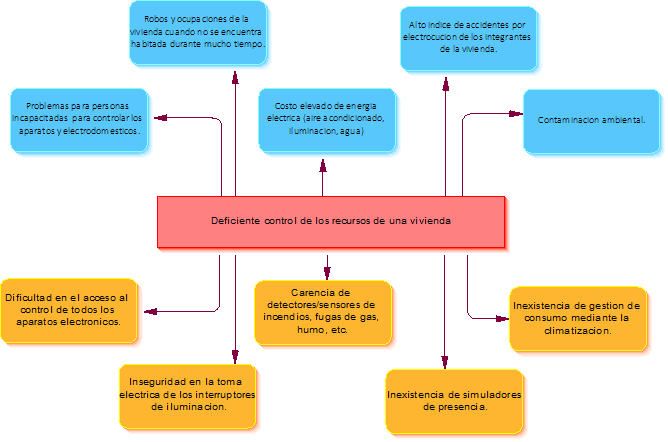
\includegraphics[width=0.9\linewidth]{imagenes/ap.png}
			\caption{Árbol de Problemas (Elaboración Propia)}
			\label{arbolProblema} 
			% Label: es para realizar referencias cruzadas, 
			% notar que se escribe todo junto y sin acentos.
		\end{figure}
		\subsection{Descripción del Problema}
		El problema central donde se enfocara el proyecto, es la exagerada utilización de los recursos energéticos de una vivienda. También está la dificultad de las personas de la tercera edad y niños, difícilmente pueden acceder al control de estos electrodomésticos, y si lo hiciera, lo lograría con el riesgo de dañar su integridad física.

	\section{Propuesta de solución}
	Para resolver todos los problemas  vistos anteriormente en el árbol de problemas se hará que cada una de ellas sea solucionada indirectamente. Para eso se verá el árbol de medios y fines.
	
		\subsection{Árbol de medios y  fines}
			El árbol de medios y fines no es más  que el árbol de problemas pero transformada desde una vista positiva de los problemas ya vistos.  De  esta manera las  causas serán objetivos a cumplir, el problema central será el objetivo meta y los efectos serán los resultados a obtener, como se pude apreciar en la Figura \ref{arbolSolucion} para su mejor comprensión.
 		\begin{figure}[ht]
			\centering
			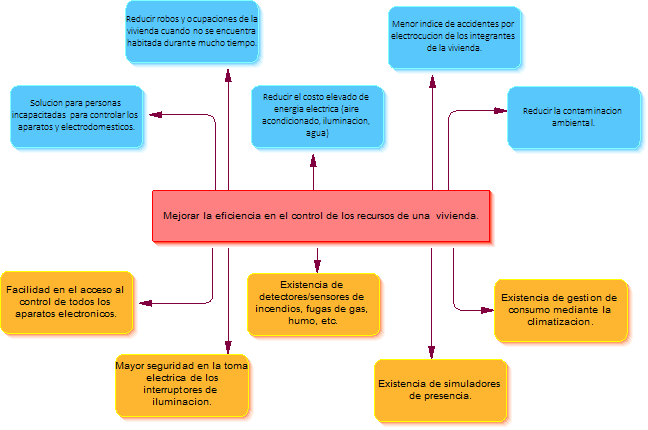
\includegraphics[width=0.9\linewidth]{imagenes/aMF.png}
			\caption{Árbol de Solucion (Elaboración Propia)}
			\label{arbolSolucion} 
			% Label: es para realizar referencias cruzadas, 
			% notar que se escribe todo junto y sin acentos.
		\end{figure}
	\section{Objetivo general}
	Implementación de un sistema domótico para el control de los recursos domésticos en vivienda unifamiliar.

	\section{Objetivos específicos}

	Los objetivos específicos que contribuirán a desarrollar el \textit{objetivo general} del trabajo son los siguientes:

	\begin{itemize}
		\item Monitoreo de la vivienda mediante sensores de presencia, temperatura, humedad y lluvia.
		\item Facilidad en el acceso al control en tiempo real de todos los aparatos eléctricos.
		\item Aplicar de NodeJS para montar un servidor con el cual se realizara el control en tiempo real de los recursos de la vivienda.
		\item Implementación de un simulador de presencia para la seguridad de la vivienda.
	\end{itemize}

	\section{Justificación}
	Con la realización del sistema de control domótico para los habitantes de la vivienda se le asegura un aumento del confort, de la seguridad, del ahorro energético y de las facilidades de comunicación, haciendo uso de las nuevas tecnologías de comunicación y teléfonos inteligentes.
	\section{Alcance}
	Dirige los recursos de una vivienda  como el control de encendido y apagado de las luces también monitorea la vivienda como ser los datos de  temperatura, humedad y gas. Todo esto se realiza  haciendo uso del sistema de Control que interactúa  a través de una página web que está conectada mediante una red local o global como el internet estando dentro de la vivienda o de manera remota. Controlando en tiempo real, para que los  usuarios  puedan ver los cambios al momento de realizarse.
	
Para el mejor control de los dispositivos de la vivienda se hará uso de las placas de micro-controladores Arduino conjuntamente de los sensores de temperatura, humedad, lluvia y detectores de gas y humo.

No se tendrán cuentas de usuario ni restricciones para el acceso al sistema, no se   garantiza el estado de los electrodomésticos y otros recursos por el manejo inapropiado del sistema.



\chapter{DOMÓTICA}	
	\section{Introducción}
	El concepto domótica se refiere a la automatización y control (encendido / apagado, apertura / cierre y regulación) de aparatos y sistemas de instalaciones eléctricas y electrotécnicos (iluminación, climatización, persianas y toldos, puertas y ventanas motorizados, el riego, etc.) de forma centralizada y/o remota. El objetivo del uso de la domótica es el aumento del confort, el ahorro energético y la mejora de la seguridad personal y patrimonial en la vivienda. \citep{morales2011} 
	
	%ejemplo de cita 'En el texto' sin parentesis, para citar con parentesis usar \citep{}
	\section{Aspectos principales}
	Los servicios que ofrece la domótica se pueden agrupar en cuatro aspectos principales:\citep{moya2004}
	\begin{itemize}
		\item En el ámbito del ahorro energético.
		\item En el ámbito del nivel de confort.
		\item En el ámbito de la protección patrimonial.
		\item En el ámbito de las comunicaciones.
	\end{itemize}
	\subsection{En el ámbito del ahorro energético}
	El ahorro energético es un pilar fundamental en la domótica, ya que con la automatización de diferentes recursos dentro la vivienda se asegura el consumo justo de la energía eléctrica. Para este propósito se tienen los siguientes puntos  más sobresalientes:
	\begin{itemize}
		\item Climatización: Aspectos que se relacionan con el clima y estaciones del año.
			\subitem Programación: La libertad de poder realizar el control de la manera que uno lo prefiera.
			\subitem Zonificación: Adecuarse a una estación del año.
		\item Gestión eléctrica:
			\subitem Racionalización de cargas eléctricas: Desconexión de equipos de uso no prioritario.
			\subitem Gestión de tarifas: Derivando el funcionamiento de algunos aparatos a horas de tarifa reducida.
			\subitem Uso de energías renovables: energía eólica y la energía termosolar. 
	\end{itemize}	
	\subsection{En el ámbito del nivel de confort}
	Conlleva todas las actuaciones que se
puedan llevar a cabo que mejoren el confort en una vivienda.
Dichas actuaciones pueden ser de carácter tanto pasivo,
como activo o mixtas. 
	\begin{itemize}
		\item Iluminación:La mayor parte de los recursos en una vivienda son las luces.
			\subitem Automatización del apagado/ encendido en cada punto de luz.
			\subitem Regulación de la iluminación según el nivel de luminosidad ambiente.
		\item Automatización de todos los distintos sistemas dotándolos de control eficiente y de fácil manejo:
			\subitem Sistemas de telefonía/energía eléctrica.
			\subitem Redes de gas/agua.
			\subitem Equipos electrónicos.
		\item Integración del portero al teléfono, o del video-portero al televisor:
			\subitem Recepción de personas en la puerta de la vivienda.
		\item Control vía Internet:
			\subitem Aplicaciones para teléfonos inteligentes.
		\item Gestión Multimedia y del recreo electrónico:
			\subitem Manipulación de los equipos de sonido y cine en casa.
		\item Generación de macros y programas de forma sencilla para el usuario:
			\subitem Sistemas de control domótico.
	\end{itemize}
	\subsection{En el ámbito de la protección patrimonial (seguridad)}
	Consiste en una red de seguridad encargada de proteger tanto los Bienes Patrimoniales y la seguridad personal.
		\begin{itemize}
		\item Simulación de presencia:
			\subitem Escenarios para simular presencia en la vivienda.
		\item Detección de conatos de incendio, fugas de gas, escapes de agua.
			\subitem Actuadores de cierre y apagado:
			\subitem Notificación de los problemas a los habitantes de la vivienda.
		\item Alerta médica. Tele-asistencia:
			\subitem Marcado automático a emergencias.
		\item Cerrar  persianas en forma puntual y seguro:
			\subitem De acuerdo al clima o definidos por el habitante de la vivienda.
		
		\end{itemize}
	\subsection{En el ámbito de las comunicaciones}
	Este aspecto se observa la relación del sistema domótico con el habitante de la vivienda, la forma de comunicarse  fuera  o en el interior, recibir las señales y poder realizar acciones.
		\begin{itemize}
		\item Ubicuidad en el control tanto externo como interno.
		\item Transmisión de alarmas.
		\item Intercomunicaciones.		
		\end{itemize}
	\section{Estructura de una Instalación Domótica}
	La amplitud de una solución de domótica puede variar desde un único dispositivo, que realiza una sola acción, hasta amplios sistemas que controlan prácticamente todas las instalaciones dentro de la vivienda\citep{casadomo:2017:Misc}. Los distintos dispositivos de los sistemas de domótica se pueden clasificar en los siguientes grupos:
		\begin{itemize}
		\item Controlador: Los controladores son los dispositivos que gestionan el sistema según la programación y la información que reciben. Puede haber un solo controlador, o varios distribuidos por el sistema. 
		\item Actuador: El actuador es un dispositivo capaz de ejecutar y/o recibir una orden del controlador y realizar una acción sobre un aparato o sistema (encendido/apagado, subida/bajada, apertura/cierre, etc.).
		\item Sensor: El sensor es el dispositivo que monitoriza el entorno captando información que transmite al sistema (sensores de agua, gas, humo, temperatura, viento, humedad, lluvia, iluminación, etc.). 
		\item Bus: Es bus es el medio de transmisión que transporta la información entre los distintos dispositivos por un cableado propio, por la redes de otros sistemas (red eléctrica, red telefónica, red de datos) o de forma inalámbrica. 
		\item Interface: Los interfaces refiere a los dispositivos (pantallas, móvil, Internet, conectores) y los formatos (binario, audio) en que se muestra la información del sistema para los usuarios (u otros sistemas) y donde los mismos pueden interactuar con el sistema.		
		\end{itemize}
		Es preciso destacar que todos los dispositivos del sistema de domótica no tienen que estar físicamente separados, sino varias funcionalidades pueden estar combinadas en un equipo. Por ejemplo en la Figura \ref{domotica_componentes} se muestra un equipo de Central de Domótica, que puede ser compuesto por un controlador, actuadores, sensores y varios interfaces. 

		\subsection{Actuación los Sistemas de Domótica}
		Los sistemas de domótica actúan sobre, e interactúan con, los aparatos y sistemas eléctricos de la vivienda según:
		\begin{itemize}
		\item El programa y su configuración.
		\item La información recogida por los sensores del sistema.
		\item La información proporcionada por otros sistemas interconectados.
		\item La interacción directa por parte de los usuarios.		
		\end{itemize}
		\begin{figure}[ht]
			\centering
			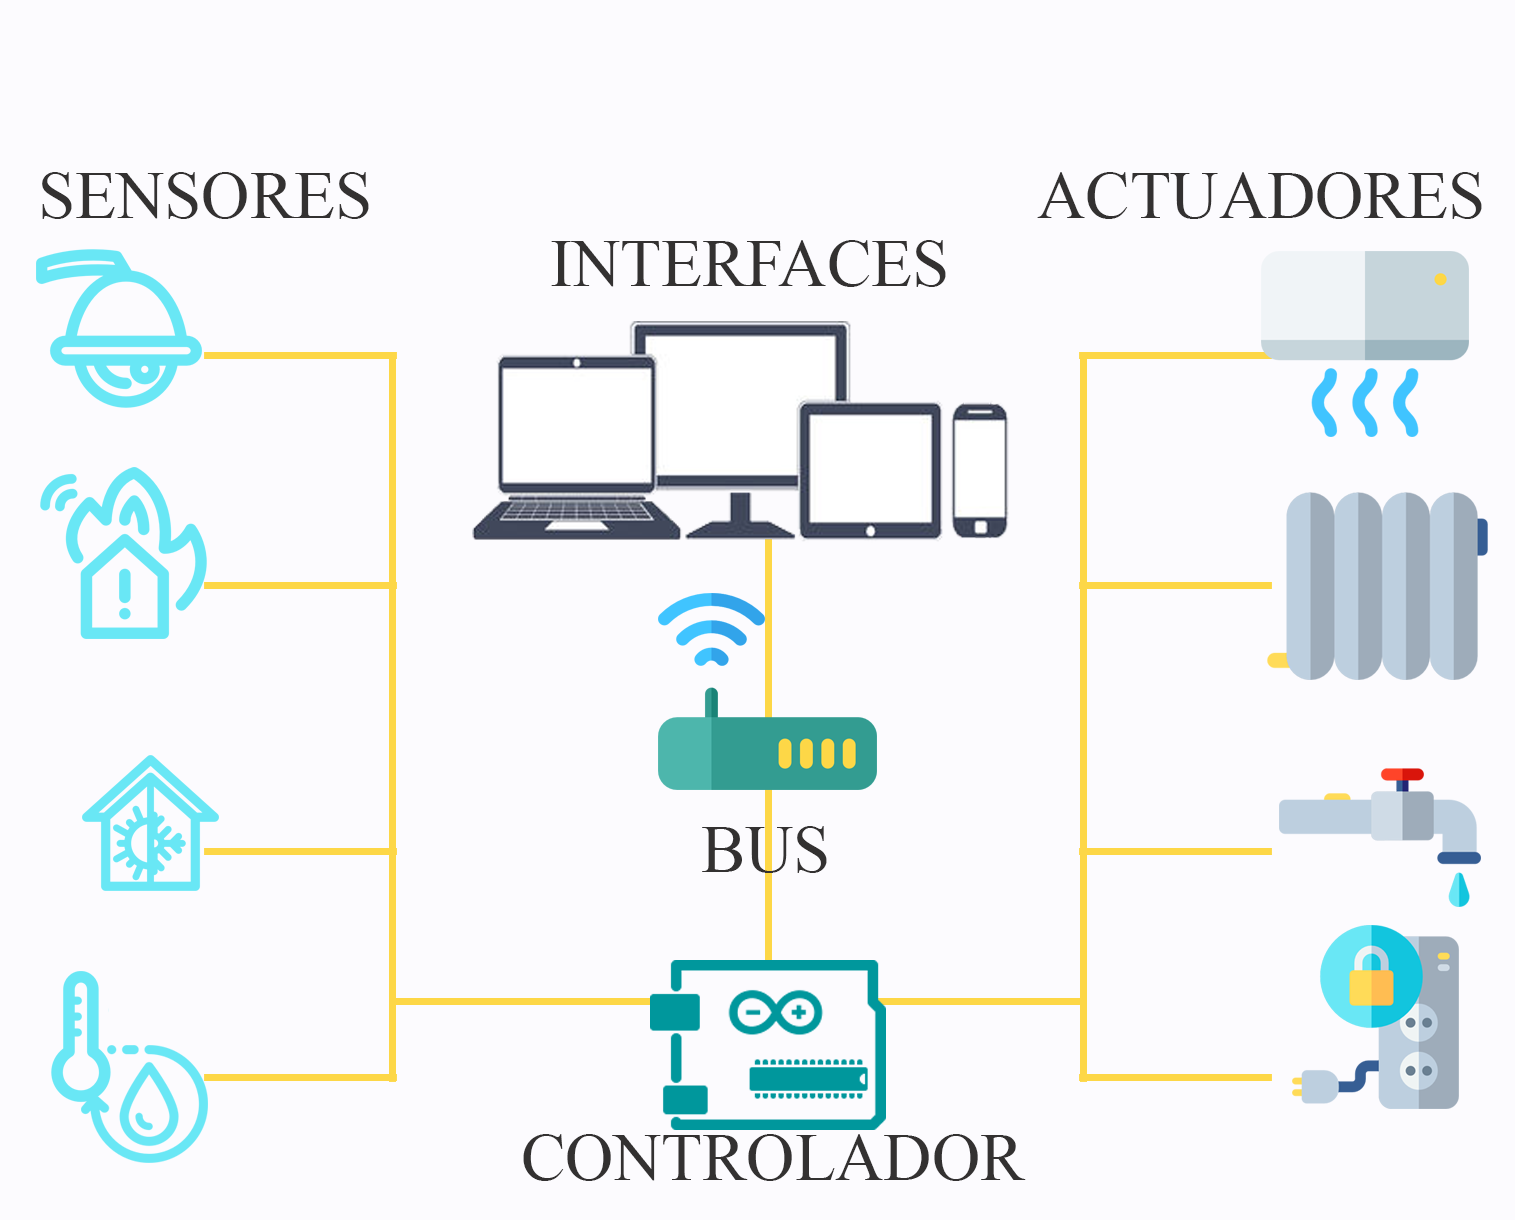
\includegraphics[scale=0.2]{imagenes/domotica_componentes.png}
			\caption{Dispositivos de sistema domotico (Elaboración Propia)}
			\label{domotica_componentes} 
		\end{figure}
		\section{Arquitectura de un Sistema de Domótica }
		La arquitectura de los sistemas de domótica hace referencia a la estructura de su red. La clasificación se realiza en base de donde reside la “inteligencia” del sistema domótico\citep{Pedro2009}. Las principales arquitecturas son: 
		\begin{itemize}
		\item Arquitectura Centralizada.- En un sistema de domótica de arquitectura centralizada, un controlador centralizado, envía la información a los actuadores e interfaces según el programa, la configuración y la información que recibe de los sensores, sistemas interconectados y usuarios. Como se aprecia en la Figura \ref{fig:centralizada}.
		\item Arquitectura Descentralizada – En un sistema de domótica de Arquitectura Descentralizada, observe la Figura \ref{fig:descentralizada} hay varios controladores, interconectados por un bus, que envía información entre ellos y a los actuadores e interfaces conectados a los controladores, según el programa, la configuración y la información que recibe de los sensores, sistemas interconectados y usuarios.  
		\item Arquitectura Distribuida - En un sistema de domótica de arquitectura distribuida, en la Figura \ref{fig:distribuida}, se puede apreciar que  cada sensor y actuador es también un controlador capaz de actuar y enviar información al sistema según el programa, la configuración, la información que capta por si mismo y la que recibe de los otros dispositivos del sistema.
		\item Arquitectura Híbrida / Mixta – En un sistema de domótica de arquitectura híbrida (también denominado arquitectura mixta) se combinan las arquitecturas de los sistemas centralizadas, descentralizadas y distribuidas.Observe la Figura \ref{fig:mixta} que a la vez que puede disponer de un controlador central o varios controladores descentralizados, los dispositivos de interfaces, sensores y actuadores pueden también ser controladores (como en un sistema “distribuido”) y procesar la información según el programa, la configuración, la información que capta por si mismo, y tanto actuar como enviarla a otros dispositivos de la red, sin que necesariamente pasa por otro controlador.			
		\end{itemize}
		%imagenes  de las distintos tipos de arquitectura de Domotica.
			%\begin{figure}[h]
			%\centering
			%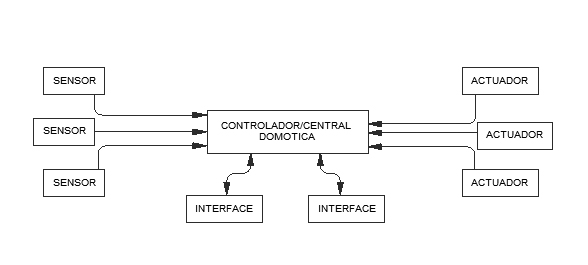
\includegraphics[scale=0.7]{imagenes/CETRALIZADA_.jpg}
			%\caption{Arquitectura domótica centralizada. (Elaboración Propia)}
			%\label{} 
			%\end{figure}		    
		    %\begin{figure}[h]
			%\centering
		%	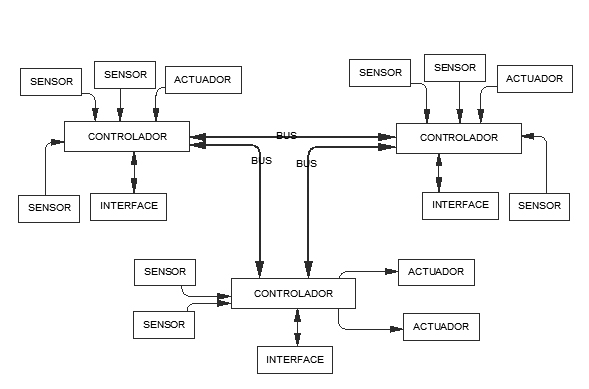
\includegraphics[scale=0.7]{imagenes/DESCENTRALIZADA_.jpg}
		%	\caption{Arquitectura domótica descentralizada. (Elaboración Propia)}
		%	\label{descentralizada} 
		%	\end{figure}
		%	\begin{figure}[h]
		%	\centering
		%	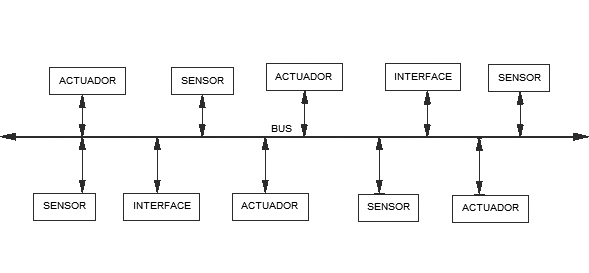
\includegraphics[scale=0.7]{imagenes/DISTRIBUIDA_.jpg}
		%	\caption{Arquitectura domótica distribuida. (Elaboración Propia)}
		%	\label{distribuida} 
		%	\end{figure}
		%	\begin{figure}[h]
		%	\centering
		%	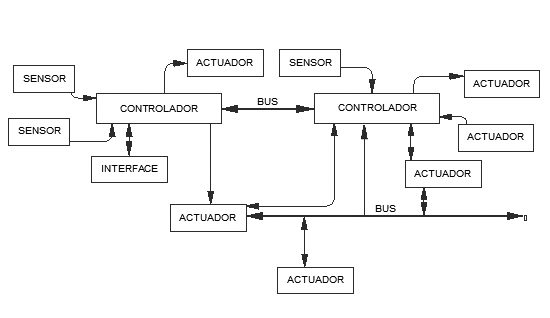
\includegraphics[scale=0.7]{imagenes/MIXTA_.jpg}
		%	\caption{Arquitectura domótica mixta. (Elaboración Propia)}
		%	\label{mixta} 
		%	\end{figure}
%segunda  firura
		\begin{figure}
    \centering
    \begin{subfigure}[b]{0.5\textwidth}
        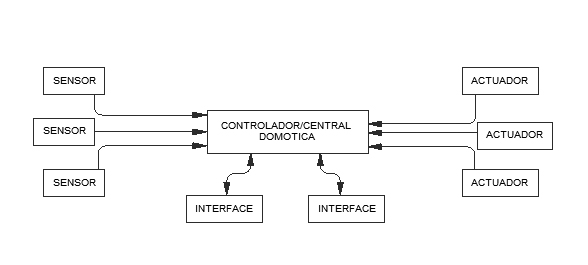
\includegraphics[width=\textwidth]{imagenes/CETRALIZADA_.jpg}
        \caption{Arquitectura domótica centralizada. }
        \label{fig:centralizada}
    \end{subfigure}
    ~ %add desired spacing between images, e. g. ~, \quad, \qquad, \hfill etc. 
      %(or a blank line to force the subfigure onto a new line)
    \begin{subfigure}[b]{0.44\textwidth}
        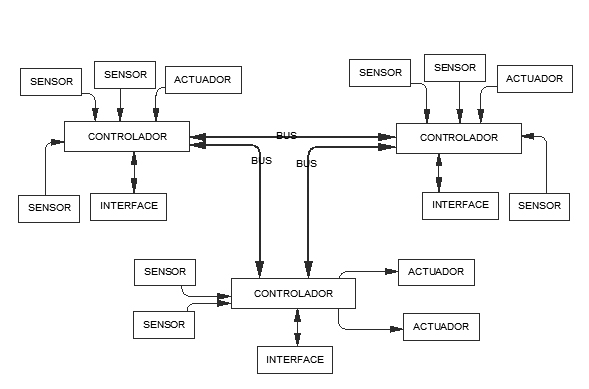
\includegraphics[width=\textwidth]{imagenes/DESCENTRALIZADA_.jpg}
        \caption{Arquitectura domótica descentralizada.}
        \label{fig:descentralizada}
    \end{subfigure}
    ~ %add desired spacing between images, e. g. ~, \quad, \qquad, \hfill etc. 
    %(or a blank line to force the subfigure onto a new line)
    \begin{subfigure}[b]{0.5\textwidth}
        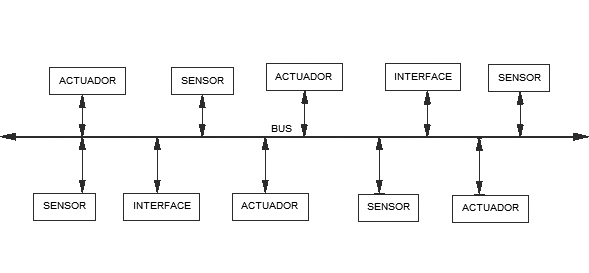
\includegraphics[width=\textwidth]{imagenes/DISTRIBUIDA_.jpg}
        \caption{Arquitectura domótica distribuida. }
        \label{fig:distribuida}
    \end{subfigure}
     ~ %add desired spacing between images, e. g. ~, \quad, \qquad, \hfill etc. 
    %(or a blank line to force the subfigure onto a new line)
    \begin{subfigure}[b]{0.5\textwidth}
        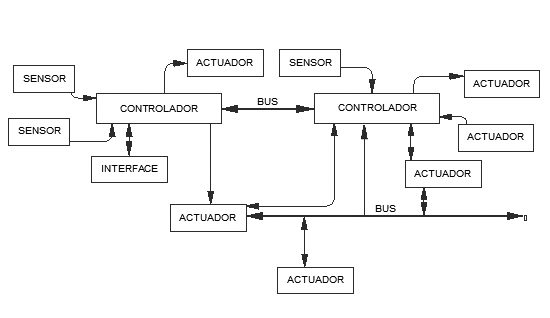
\includegraphics[width=\textwidth]{imagenes/MIXTA_.jpg}
        \caption{Arquitectura domótica mixta. }
        \label{fig:mixta}
    \end{subfigure}
    \caption{Arquitectura domótica(Elaboración Propia)}\label{fig:shelter}
\end{figure}
		\section{Medios de Transmisión / Bus}
		El medio de transmisión de la información, interconexión y control, entre los distintos dispositivos de los sistemas de domótica puede ser de varios tipos \citep{casadomo:2017:Misc}. Los principales medios de transmisión son: 
		\begin{itemize}
		\item Cableado Propio – La transmisión por un cableado propio es el medio más común para los sistemas de domótica, principalmente son del tipo: par apantallado, par trenzado (1 a 4 pares), coaxial o fibra óptica.
		\item Cableado Compartido – Varios soluciones utilizan cables compartidos y/o redes existentes para la transmisión de su información, por ejemplo la red eléctrica (corrientes portadoras), la red telefónica o la red de datos.  
		\item Inalámbrica – Muchos sistemas de domótica utilizan soluciones de transmisión inalámbrica entre los distintos dispositivos, principalmente tecnologías de radiofrecuencia o infrarrojo. 
		\end{itemize}
		Cuando el medio de transmisión esta utilizado para transmitir información entre dispositivos con la función de “controlador” también se denomina “Bus”. El bus también se utiliza muchas veces para alimentar a los dispositivos conectados a él (por ejemplo European Instalation Bus – EIB). 
		\section{Sistemas Domóticos}
		Existen diferentes tecnologías o estándares de domótica que se aplican para la implementación de dispositivos y la red de comunicación, entre los que cabe señalar:
		\begin{itemize}
		\item Sistemas Domóticos Ad Hoc 
Estos sistemas están pensados para aplicaciones determinadas y su configuración es muy limitada, como por ejemplo el control de intensidad de una luminaria, el control de riego por temporizador, el encendido de luminarias activadas por sensor de movimiento y así un número de posibles ejemplos para casos concretos. Pero, en definitiva serán pocos elementos, unos cercanos a otros que posiblemente podamos encontrar en estructuras centralizadas con conexión en estrella basadas en bus.
La funcionalidad de los sistemas está limitada a la programación establecida por fábrica, dejando poco margen de configuración por parte del usuario, tan solo tendrá libertad para definir unos pocos parámetros, por ejemplo, en un temporizador de regadío, el horario de encendido y de apagado.
Debido a que están pensados para aplicaciones determinadas encontraremos en el mercado los elementos Ad Hoc especializados en algún tipo de aplicación: seguridad, control de clima, alarmas, confort, ahorro energético, etc. Una característica importante es que los elementos no pueden comunicarse entre sí, sin embargo, es viable insertar elementos ad hoc, mediante adaptadores, en un sistema domótico que utilice una de las tres restantes técnicas, pudiendo ser controlado\citep{Pedro2009}.
		\item Sistemas Domóticos sobre Red Eléctrica de Baja Tensión
En este tipo de instalaciones domóticas, en Redes Eléctricas de Baja Tensión, también conocidas como Power Line (PL), el medio de transmisión es el cableado de la red eléctrica de baja tensión (220 VAC). La transmisión es digital para lo cuál se requiere que la onda sinusoidal 20 sea lo más limpia posible, como máximo tenga una distorsión del 10 \% sobre la tensión eficaz de 220 VAC y en frecuencia +/- 0.5 Hz. sobre los 50 Hz.
Al emitir una señal de radiofrecuencia el sistema ha estar homologado para cumplir las normas que eviten que dicha señal interfiera en la señal del suministro eléctrico. Además, al ser aditiva dicha interferencia, proveniente de los diversos sistemas domóticos en paralelo, hay que atender a este detalle a la hora de la planificación del proyecto domótico. Aunque normalmente con los sistemas homologados y un buen diseño, en general, los sistemas PL introducen poca interferencia de radiofrecuencia.
Otro detalle a tener en cuenta en los sistemas domóticos PL es la impedancia. Ésta genera una disminución de la tensión como consecuencia del decremento de la impedancia, causada por el aumento de la capacidad electrostática (C). Estos pequeños cambios resistivos son detectados por los sistemas domóticos y deben adaptarse dinámicamente a ellos.
Con estos puntos a tener en cuenta la aplicación domótica PL no se debe utilizar, por normativa, en los casos siguientes: a la hora de monitorizar equipos médicos, conectar varios edificios, en redes eléctricas donde estén conectadas maquinarias que sobrepasen los límites de interferencia radioeléctrica (generalmente motores de potencia), cuando exista transformadores en la red eléctrica, si la línea de red eléctrica es utilizada por sistemas que utilicen la banda de 105,6 kHZ. – 115,2 kHZ. y finalmente, cuando no se asegure los límites 220c +/- 10 \% y 50 Hz. +/- 0,5 Hz\citep{Pedro2009}.
		\item Técnica sobre Radio Frecuencia
Los elementos empleados para esta técnica utilizan como medio de transmisión el radioeléctrico. Cada sensor y actuador lleva integrado un dispositivo transmisor y receptor.
Un solo receptor (o varios, si existen obstáculos insalvables o la vivienda es amplia) es el que recibe las señales de los sensores para procesarla y emitirla a los actuadores.
La comodidad de esta técnica es que no hace falta ninguna obra de acometida para la instalación. Incluso pueden adherirse a cristales (como mamparas) haciendo al sistema muy versátil.
La frecuencia utilizada para la transmisión aún no está estandarizada, por ejemplo, Jung, utiliza 433 MHz con una potencia más baja que la empleada en la telefonía móvil. Dicha frecuencia permite una transmisión de 1000 bits/s. La modulación utilizada es ASK (Amplitude Shift Keying). Un “1” ó “0” se asocia a un nivel distinto de señal que se modula con la portadora de 433 MHz. El alcance dependerá de los obstáculos que se encuentren, normalmente cuando el espacio es diáfano la distancia es de 300 m. decreciendo a 50 m. cuando existen obstáculos\citep{Pedro2009}.
		\end{itemize}
		\subsection{ Los Protocolos de Domótica}
		Los protocolos de comunicación son los procedimientos utilizados por los sistemas de domótica para la comunicación entre todos los dispositivos con la capacidad de “controlador”. 
Existen una gran variedad de protocolos, algunos específicamente desarrollados para la domótica y otros protocolos con su origen en otros sectores, pero adaptados para los sistemas de domótica. Los protocolos pueden ser del tipo estándar abierto (uso libre para todos), estándar bajo licencia (abierto para todos bajo licencia) o propietario (uso exclusivo del fabricante o los fabricantes propietarios)\citep{moya2004}.
 
No se puede entender la domótica, sin conocer el protocolo de comunicaciones, como lenguaje de comunicación del Sistema Domótico. A través del protocolo se comunican los diversos dispositivos que componen la red domótica, de los cuales sobresalen los protocolos:
		\begin{itemize}
		\item Propietarios o cerrados.- Son protocolos específicos de una marca en particular y que solo son usados por dicha marca. Pueden ser variantes de Protocolos Estándar.
Son protocolos cerrados de manera que solo el fabricante puede realizar mejoras y fabricar dispositivos que “hablen” el mismo idioma.
Esto protege los derechos del fabricante, pero limita la aparición de continuas evoluciones en los sistemas domóticos, con lo que, a medida que los sistemas con protocolo estándar se van desarrollando, van ganando cuota de mercado a los sistemas de protocolo propietario.
Otro problema que tienen es: la vida útil del sistema domótico, en un sistema propietario que depende en gran medida de la vida de la empresa y de la política que siga, si la empresa desaparece, el sistema desaparece y las instalaciones se quedan sin soporte ni recambios.
		\item Estándar o Abiertos.- Son protocolos definidos entre varias compañías con el fin de unificar criterios.
Se los conoce como abiertos (open systems), es decir, que no existen patentes sobre el protocolo de manera que cualquier fabricante puede desarrollar aplicaciones y productos que lleven implícito el protocolo de comunicación.
En un sistema estándar, si una empresa desaparece o deja de sacar productos al mercado, no afecta demasiado ya que hay otros productos en el mercado que cubren ese aspecto.

		\end{itemize}
		\subsection{Tecnologías y estándares}
		Algunas tecnologías siguen presentes hasta el momento y se aplican en los sistemas domóticos actuales \citep{herrera2005}. Los protocolos estándar para aplicaciones domóticas más extendidos en la actualidad son: KNX, Lonworks y X10 como se observa en la  Figura \ref{estandaresDomoticos}.
		\begin{itemize}
		\item X-10: EE.UU finales de los 70.
		\item EHS (European Home System): 1992 Unión Europea.
		\item EIB (European Installation Bus).
		\item BatiBUS.
		\item KONNEX: EHS + EIB + BatiBUS.
		\item BIODOM: desarrollado por españoles.
		\item BACnet (de Building Automation and Control Networks).
		\end{itemize}
		\begin{figure}[h]
		\centering
		
\includegraphics[scale=0.7]{imagenes/estandares_internacionales_de_domotica2.png}
		\caption{Estandares Internacionalesde Domotica. (Elaboración Propia)}
		\label{estandaresDomoticos} 
		\end{figure}
		\subsection{Funcionamiento De Un Sistema Domótico}
		La configuración de un sistema domótico está íntimamente ligada a los procedimientos de transmisión de información que posibilitan el diálogo entre dichos periféricos y la unidad central. Los terminales (radiadores de calefacción, electrodomésticos, puntos de luz, etc.). Suelen ser equipos convencionales a los que se aporta una inteligencia o capacidad de comunicación a través de una interfaz. Los elementos de campo comprenden todo el conjunto de sensores que permiten convertir una magnitud física en señal eléctrica, y los actuadores u órganos de mando, capaces de transformar una señal eléctrica en una acción sobre el entorno físico.
		
Todos los elementos de campo envían y reciben señales a través de una red de comunicaciones (bus domótico), para comunicarse entre ellos y con la unidad central encargada de gestionar los intercambios de información. Estas señales de control están codificadas de una determinada forma (protocolos de comunicación), por lo que se necesitan unos elementos que pasen las señales bus y, a su vez, de señales bus a señales de salida a los actuadores (relés, interruptores, etc.). Estos elementos se suelen denominar de diferentes formas: módulos de entrada/salida, acopladores, interfaces, etc.\citep{moya2004}.
\chapter{ARDUINO Y NODEJS}	
	\section{Introducción}
	Arduino es una plataforma de hardware libre, basada en una placa con un microcontrolador y un entorno de desarrollo, diseñada para facilitar el uso de la electrónica en proyectos multidisciplinares.
El hardware consiste en una placa con un microcontrolador Atmel AVR y puertos de entrada/salida. Los microcontroladores más usados son el Atmega168, Atmega328, Atmega1280, ATmega8 por su sencillez y bajo coste que permiten el desarrollo de múltiples diseños. Por otro lado el software consiste en un entorno de desarrollo que implementa el lenguaje de programación Processing/Wiring y el cargador de arranque que es ejecutado en la placa.
Arduino puede tomar información del entorno a través de sus entradas analógicas y digitales, puede controlar luces, motores y otros actuadores. El microcontrolador en la placa Arduino se programa mediante el lenguaje de programación Arduino (basado en Wiring) y el entorno de desarrollo Arduino (basado en Processing)\citep{mcroberts2011arduino}.
	\section{Programar un Arduino}
	Para programar un Arduino es necesario descargar e instalar el Arduino IDE, esta herramienta nos permite programar y subir nuestros archivos al dispositivo, el lenguaje de programación utilizado es compatible con C/C++ (a simple vista no es estrictamente C/C++ pero al momento de compilar el IDE se encarga de agregar los headers necesarios para que funcione en el dispositivo).
	
La estructura básica del lenguaje de programación de Arduino es bastante simple y se compone de al menos dos partes. Estas dos partes necesarias, o funciones, encierran bloques que contienen declaraciones, estamentos o instrucciones.
El setup() es la parte encargada de recoger la configuración y loop() es la que contiene el programa que se ejecutará cíclicamente (de ahí el término loop –bucle-). Ambas funciones son necesarias para que el programa trabaje, en la Figura \ref{estructuraArduino} se muestra la sintaxis.

La función de configuración (setup) debe contener la declaración de las variables. Es la primera función a ejecutar en el programa, se ejecuta sólo una vez, y se utiliza para configurar o inicializar pinMode (modo de trabajo de las E/S), configuración de la comunicación en serie y la inicialización de variables.
La función bucle (loop) siguiente contiene el código que se ejecutara continuamente (lectura de entradas, activación de salidas, etc.) Esta función es el núcleo de todos los programas de Arduino y la que realiza la mayor parte del trabajo.
	\begin{figure}[ht]
	\centering
	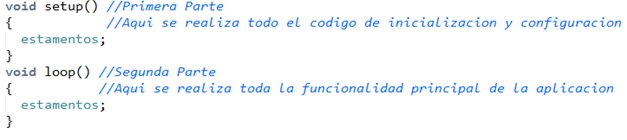
\includegraphics[scale=0.7]{imagenes/ardui.png}
	\caption{Estructura de un Programa Arduino. (Elaboración Propia)}
	\label{estructuraArduino} 
	\end{figure}

	\section{NodeJS}
	Nodejs es un entorno en tiempo de ejecución multiplataforma, de código abierto, para la capa del servidor basado en el lenguaje de programación ECMAScript, asíncrono, con I/O de datos en una arquitectura orientada a eventos por lo tanto asíncrona, basado en el motor V8 de Google. V8 es el entorno de ejecución para JavaScript creado para Google Chrome, está escrito en C++ y compila el código fuente JavaScript en código de máquina en lugar de interpretarlo en tiempo real al lado del servidor. Nodejs contiene libuv para manejar eventos asíncronos. Libuv es una capa de abstracción de funcionalidades de redes y sistemas de archivo en sistemas Windows y sistemas basados en POSIX como Linux, Mac OS X y Unix.
Además de la alta velocidad de ejecución de Javascript, la verdadera magia detrás de Nodejs es algo que se llama Bucle de Eventos (Event Loop - espera y envía eventos o mensajes). Para escalar grandes volúmenes de clientes, todas las operaciones intensivas I/O en Nodejs se llevan a cabo de forma asíncrona.
		\subsection{Gestor De Paquetes }
		Se han construido miles de bibliotecas de código abierto para Node.js, la mayoría de las cuales están alojadas la web de NPM(Node Package Manager).
Es el gestor de paquetes usado por Node para publicar, buscar, instalar y desarrollar aplicaciones. Permite compartir y reutilizar paquetes de código para ensamblarlos en nuevas y/o mejores funcionalidades para:
		\begin{itemize}
		\item Archivos del sistema I/O.
		\item Redes: DNS, HTTP, TCP, TLS/SSL, UDP.
		\item Datos binarios (buffers).
		\item Funciones criptográficas.
		\item Flujos de datos.
		\end{itemize}
		Estos módulos utilizan una API diseñada para reducir la complejidad de la escritura de aplicaciones de servidor.
Aunque NPM también puede gestionar paquetes del lado del cliente (front-end) está más enfocado a la gestión de módulos del servidor.
El gestor de paquetes NPM, no obstante, es un poquito distinto a otros gestores de paquetes que podemos conocer, porque los instala localmente en los proyectos. Es decir, al descargarse un módulo, se agrega a un proyecto local, que es el que lo tendrá disponible para incluir. Aunque cabe decir que también existe la posibilidad de instalar los paquetes de manera global en nuestro sistema.
		\subsection{Marcos de Desarrollo}
		Son entornos de trabajo que disponen de las librerías necesarias para automatizar y facilitar el desarrollo de aplicaciones.
		El scaffolding es una técnica admitida por algunos marcos modelo-vista-controlador , en los cuales el programador puede especificar cómo se puede usar la base de datos de la aplicación. El compilador o marco utiliza esta especificación, junto con plantillas de código predefinidas, para generar el código final que la aplicación puede usar para crear, leer, actualizar y eliminar entradas de la base de datos, tratando de manera efectiva las plantillas como un andamio  sobre el cual construir una aplicación más poderosa\citep{quintana2004scaffolding}.
		\begin{itemize}
		\item Generador de aplicaciones Express.- Es una herramienta del generador de aplicaciones, express-generator para crear rápidamente un esqueleto de aplicación, disponible en el gestor de paquetes. Observe la Figura  la cual es representa la estructura de directorios generada.
		\end{itemize}
		\begin{figure}[ht]
		\centering
		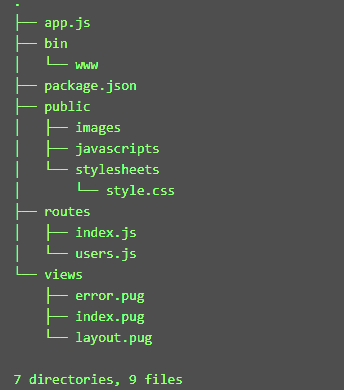
\includegraphics[scale=0.7]{imagenes/express2.png}
		\caption{Estructura de Directorios Generada con Express. (Elaboración Propia)}
		\label{estructuraExpress} 
		\end{figure}
		\subsection{Componentes para comunicación en tiempo real}
		Socketio es una librería que nos permite manejar eventos en tiempo real mediante una conexión TCP y todo ello en JavaScript. Con el cual  tenemos a nuestra disposición un nuevo protocolo que permite la interacción entre el cliente y el servidor, facilitando la transmisión de datos en tiempo real en ambas direcciones, es una comunicación bidireccional (el emisor envía un mensaje por medio de un canal al receptor, quien lo recibe y envía la retroalimentación)\citep{rai2013socket}.
		\section{Comunicación serial}
		La comunicación serial es un protocolo muy común para comunicación entre dispositivos que se incluye de manera estándar en prácticamente cualquier computadora. La comunicación serial es también un protocolo común utilizado por varios dispositivos para instrumentación; existen varios dispositivos compatibles con GPIB que incluyen un puerto RS-232. Además, la comunicación serial puede ser utilizada para adquisición de datos si se usa en conjunto con un dispositivo remoto de muestreo\citep{tamayo2009}.
		
		El concepto de comunicación serial es sencillo. El puerto serial envía y recibe bytes de información un bit a la vez. Aun y cuando esto es más lento que la comunicación en paralelo, que permite la transmisión de un byte completo por vez, este método de comunicación es más sencillo y puede alcanzar mayores distancias. Por ejemplo, la especificación IEEE 488 para la comunicación en paralelo determina que el largo del cable para el equipo no puede ser mayor a 20 metros, con no más de 2 metros entre cualesquier dos dispositivos; por el otro lado, utilizando comunicación serial el largo del cable puede llegar a los 1200 metros\citep{tamayo2009}.
		
		Típicamente, la comunicación serial se utiliza para transmitir datos en formato ASCII. Para realizar la comunicación se utilizan 3 líneas de transmisión: (1) Tierra (o referencia), (2) Transmitir, (3) Recibir. Debido a que la transmisión es asincrónica, es posible enviar datos por un línea mientras se reciben datos por otra. Existen otras líneas disponibles para realizar handshaking, o intercambio de pulsos de sincronización, pero no son requeridas. Las características más importantes de la comunicación serial son la velocidad de transmisión, los bits de datos, los bits de parada, y la paridad\citep{instruments2006}. Para que dos puertos se puedan comunicar, es necesario que las siguientes características sean iguales:
		\begin{itemize}
		\item Velocidad de transmisión (baud rate): Indica el número de bits por segundo que se transfieren, y se mide en baudios (bauds). Por ejemplo, 300 baudios representa 300 bits por segundo. Cuando se hace referencia a los ciclos de reloj se está hablando de la velocidad de transmisión. Por ejemplo, si el protocolo hace una llamada a 4800 ciclos de reloj, entonces el reloj está corriendo a 4800 Hz, lo que significa que el puerto serial está muestreando las líneas de transmisión a 4800 Hz. Las velocidades de transmisión más comunes para las lineas telefónicas son de 14400, 28800, y 33600. Es posible tener velocidades más altas, pero se reduciría la distancia máxima posible entre los dispositivos. Las altas velocidades se utilizan cuando los dispositivos se encuentran uno junto al otro, como es el caso de dispositivos GPIB.
		\item Bits de datos: Se refiere a la cantidad de bits en la transmisión. Cuando la computadora envía un paquete de información, el tamaño de ese paquete no necesariamente será de 8 bits. Las cantidades más comunes de bits por paquete son 5, 7 y 8 bits. El número de bits que se envía depende en el tipo de información que se transfiere. Por ejemplo, el ASCII estándar tiene un rango de 0 a 127, es decir, utiliza 7 bits; para ASCII extendido es de 0 a 255, lo que utiliza 8 bits. Si el tipo de datos que se está transfiriendo es texto simple (ASCII estándar), entonces es suficiente con utilizar 7 bits por paquete para la comunicación. Un paquete se refiere a una transferencia de byte, incluyendo los bits de inicio/parada, bits de datos, y paridad. Debido a que el número actual de bits depende en el protocolo que se seleccione, el término paquete se usar para referirse a todos los casos.
		\item Bits de parada: Usado para indicar el fin de la comunicación de un solo paquete. Los valores típicos son 1, 1.5 o 2 bits. Debido a la manera como se transfiere la información a través de las líneas de comunicación y que cada dispositivo tiene su propio reloj, es posible que los dos dispositivos no estén sincronizados. Por lo tanto, los bits de parada no sólo indican el fin de la transmisión sino además dan un margen de tolerancia para esa diferencia de los relojes. Mientras más bits de parada se usen, mayor será la tolerancia a la sincronía de los relojes, sin embargo la transmisión será más lenta.
		\item Paridad: Es una forma sencilla de verificar si hay errores en la transmisión serial. Existen cuatro tipos de paridad: par, impar, marcada y espaciada. La opción de no usar paridad alguna también está disponible. Para paridad par e impar, el puerto serial fijará el bit de paridad (el último bit después de los bits de datos) a un valor para asegurarse que la transmisión tenga un número par o impar de bits en estado alto lógico. Por ejemplo, si la información a transmitir es 011 y la paridad es par, el bit de paridad sería 0 para mantener el número de bits en estado alto lógico como par. Si la paridad seleccionada fuera impar, entonces el bit de paridad sería 1, para tener 3 bits en estado alto lógico. La paridad marcada y espaciada en realidad no verifican el estado de los bits de datos; simplemente fija el bit de paridad en estado lógico alto para la marcada, y en estado lógico bajo para la espaciada. Esto permite al dispositivo receptor conocer de antemano el estado de un bit, lo que serviría para determinar si hay ruido que esté afectando de manera negativa la transmisión de los datos, o si los relojes de los dispositivos no están sincronizados.
		\end{itemize}

\chapter{VIVIENDA UNIFAMILIAR}
	\section{Introducción}
	Hoy en día el crecimiento poblacional de Bolivia hace notar que muchas familias viven en la misma vivienda, lo cual rompe el concepto de vivienda unifamiliar. Si no se tiene clara el concepto de una vivienda unifamiliar, veremos algunos conceptos que lo definen como ser la familia y vivienda.
	\subsection{Familia}
	La familia es un grupo de personas formado por individuos que se unen, primordialmente, por relaciones de filiación o de pareja. El Diccionario de la Lengua Española la define, entre otras cosas, como un grupo de personas emparentadas entre sí que viven juntas , lo que lleva implícito los conceptos de parentesco y convivencia, aunque existan otros modos, como la adopción. También definida, como un conjunto de ascendientes, descendientes y demás personas relacionadas entre sí por parentesco de sangre o legal.
	
	Según la Declaración Universal de los Derechos Humanos, es el elemento natural, universal y fundamental de la sociedad, tiene derecho a la protección de la sociedad y del Estado.
	
	Los lazos principales que definen una familia son de dos tipos: vínculos de afinidad derivados del establecimiento de un vínculo reconocido socialmente, como el matrimonio que, en algunas sociedades, sólo permite la unión entre dos personas mientras que en otras es posible la poligamia, y vínculos de consanguinidad, como la filiación entre padres e hijos o los lazos que se establecen entre los hermanos que descienden de un mismo padre. También puede diferenciarse la familia según el grado de parentesco entre sus miembros.
	
	No hay consenso sobre una definición universal de la familia. La familia nuclear, fundada en la unión entre hombre y mujer, es el modelo principal de familia como tal, y la estructura difundida mayormente en la actualidad. Las formas de vida familiar son muy diversas, dependiendo de factores sociales, culturales, económicos y afectivos. La familia, como cualquier institución social, tiende a adaptarse al contexto de una sociedad.
Las familias están clasificadas en los siguientes tipos:
	\begin{itemize}
	\item Familia nuclear: formada por la madre, el padre y uno o más hijos.
	\item Familia extensa: abuelos, tíos, primos y otros parientes consanguíneos o afines.
	\item Familia monoparental: en la que el hijo o hijos viven con un solo progenitor (ya sea la madre o el padre).
	\item Familia ensamblada: Una familia ensamblada o familia reconstituida o familia mixta es una familia en la cual uno o ambos miembros de la actual pareja tiene uno o varios hijos de uniones anteriores.
	\item Familia homoparental: Se considera familia homoparental aquella donde una pareja de hombres o de mujeres se convierten en progenitores de uno o más niños.
	\item La familia de padres separados: en la que los padres se niegan a vivir juntos; no son pareja pero deben seguir cumpliendo su rol de padres ante los hijos por muy distantes que estos se encuentren.
	\end{itemize}
	 En el Estado Plurinacional de Bolivia, 45,5 \% de los hogares está conformado por el jefe de hogar, cónyuge e hijo(s) (hogar nuclear completo), mientras que 10,9 \% está integrado por el jefe/a de hogar sin cónyuge, con la presencia de hijo(s) (hogar monoparental), Segun el Instituto Nacional de Estadística (INE). Observe el Figura \ref{ine} representa la tipologia de los hogares en bolivia encuesta del año 2015. 

A nivel nacional, existen aproximadamente 3.012.000hogares, de los cuales 2.036.000 se encuentran en el área urbana y 976.000 en el área rural, según la Encuesta de Hogares 2015. El tamaño medio del hogar es de 3,6 personas sin considerar a trabajadoras del hogar\citep{bolivia2012instituto}.
		\begin{figure}[ht]
		\centering
		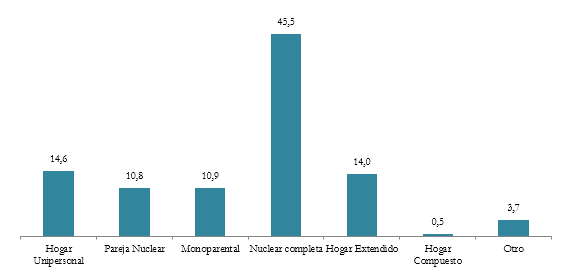
\includegraphics[scale=0.9]{imagenes/familia1.png}
		\caption{Tipología De Hogares, Encuesta De Hogares 2015. (Instituto Nacional de Estadística)}
		\label{ine} 
		\end{figure}
	\subsection{Vivienda y Hogar}
	La vivienda, es un edificio cuya principal función es ofrecer refugio y habitación a las personas, protegiéndolas de las inclemencias climáticas, el frío de la noche, del calor de algunos días y de otras amenazas naturales. La primera función de la vivienda es proporcionar un espacio seguro y confortable para resguardarse. El clima condiciona en gran medida tanto la forma de la vivienda como los materiales con que se construye y hasta las funciones que se desarrollan en su interior. 
	
La palabra hogar se usa para designar a un lugar donde un individuo o grupo habita, creando en ellos la sensación de seguridad y calma. En esta sensación se diferencia del concepto de casa, que sencillamente se refiere a la vivienda física. La palabra hogar proviene del lugar donde se encendía el fuego, a cuyo alrededor se reunía la familia para calentarse y alimentarse. Se aplica también a todas aquellas instituciones residenciales que buscan crear un ambiente hogareño, por ejemplo: hogares de retiros, hogares de crianza, etc.
	\section{Definición}
	La definición de este tipo de casa puede variar entre jurisdicciones u organismos estadísticos, y sabiendo los puntos anteriores previamente vistos lo definimos como:
	
	Una sola familia (hogar, casa o vivienda) significa que el edificio está generalmente ocupado por un solo hogar o la familia, y se compone de una sola unidad de vivienda o habitación. Se excluye, sin embargo, cualquier alojamiento a corto plazo (hoteles, moteles, casas de huéspedes), alojamiento de alquiler a gran escala (internados, apartamentos) y de las viviendas colectivas.
	
La mayoría de las viviendas unifamiliares se construyen en lotes más grandes que la propia estructura, añadiendo un área que rodea la casa, que comúnmente se llama un patio o un jardín, con un garaje y entrada. 
	\section{Tipos de viviendas}
	Las comparaciones respecto al tipo de unidad de vivienda y su organización interior, su agrupamiento y
densidad tienen implicancias en los estilos de vidade los usuarios. Las tipologías
arquitectónicas, determinan las caracteristicas de cada una de estas viviendas:
		\begin{itemize}
		\item Unifamiliar aislada o exenta: Es aquel edificio habitado por una única familia que no está en contacto físico con otras edificaciones como se aprecia en la Figura \ref{fig:aislada}. Normalmente están rodeadas por todos sus lados por un terreno perteneciente a la vivienda, en el que se suele instalar un jardín, la vivienda puede tener uno, varios o todos sus lados alineados con las calles públicas.
		\item Unifamiliar pareada: En este caso, se construyen dos viviendas unifamiliares que exteriormente están en contacto, aunque en su distribución interior son totalmente independientes, teniendo cada una de ellas su propio acceso desde la vía pública enla Figura \ref{fig:pareada}  se tiene un ejemplo.
		\item Unifamiliar adosada: Similar a la pareada, pero esta vez cada vivienda está en contacto con otras dos (una a cada lado). Este tipo de viviendas se suelen caracterizar por tener una planta estrecha y alargada y por la presencia de ventanas únicamente en los extremos de la casa como se observa en la Figura \ref{fig:adosada} donde hay dos columnas de viviendas.
		\end{itemize}
	%casas  firura
	\begin{figure}[ht]
    \centering
    \begin{subfigure}[b]{0.44\textwidth}
        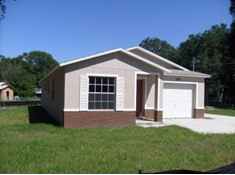
\includegraphics[width=\textwidth]{imagenes/aislada.png}
        \caption{Vivienda unifamiliar aislada. }
        \label{fig:aislada}
    \end{subfigure}
    ~ %add desired spacing between images, e. g. ~, \quad, \qquad, \hfill etc. 
      %(or a blank line to force the subfigure onto a new line)
    \begin{subfigure}[b]{0.44\textwidth}
        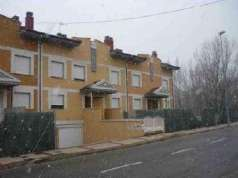
\includegraphics[width=\textwidth]{imagenes/pareada.png}
        \caption{Vivienda unifamiliar pareada.}
        \label{fig:pareada}
    \end{subfigure}
    ~ %add desired spacing between images, e. g. ~, \quad, \qquad, \hfill etc. 
    %(or a blank line to force the subfigure onto a new line)
    \begin{subfigure}[b]{0.5\textwidth}
        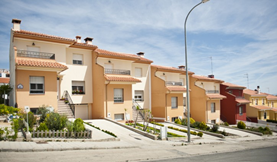
\includegraphics[width=\textwidth]{imagenes/adosada.png}
        \caption{Vivienda unifamiliar adosadas. }
        \label{fig:adosada}
    \end{subfigure}
    \caption{Tipos de Vivienda Unifamiliar(Elaboración Propia)}\label{fig:viviendas}
\end{figure}

	\section{Integrantes de una Vivienda Unifamiliar}
	Familia conviviente formada por los miembros de un único núcleo familiar, el grupo formado por los miembros de una pareja y/o sus hijos como se observa en la Figura \ref{family}. Las definiciones más amplias consideran en un núcleo familiar tanto a los grupos formados por dos adultos emparejados, con o sin hijos, como a los formados por un adulto con uno o varios hijos. Algunas definiciones más restrictivas la reducen a los casos en los que están presentes los dos progenitores.
	
	\subsection{Roles de los Integrantes}
	En el estudio de las familias, conocer cuál es la estructura familiar es uno de los pasos iniciales. Conocer el rol que cumplen cada uno de los integrantes de la familia será importante para tener una mejor visión del funcionamiento familiar.
	
La familia está organizada según el orden jerárquico en que se disponen sus miembros, donde cada posición le confiere obligaciones y prerrogativas delimitadas por reglas concretas las cuales contribuyen a vincular el funcionamiento de la familia con los fines del grupo familiar.En la familia sus miembros pueden ubicarse en el puesto de padre, madre, hijo, hermano, abuelo. Acontinuaciòn se hace mencion de los roles mas sobresalientes:
		\begin{itemize}
		\item Rol Materno.- Los psicoanalistas están de acuerdo en la concepción clínica de lo que constituye “un buen ejercicio maternal”. La madre debe constituirse en un “medio aprovisionador total” del niño y esta provisión consiste en algo más que la mera satisfacción de necesidades fisiológicas. La madre debe realizar todo lo que el niño es incapaz de hacer por sí mismo: alimentación, vestido, higiene y transporte, añadiendo a la atención maternal un contenido afectivo seguro; es un hecho emocional que se integra y unifica con el hecho físico.
		\item Rol Paterno.- La presencia de la figura paterna, está relacionada con la misión del padre en el seno de la familia, y en particular, respecto a la relación que ha de establecer con el hijo. La misión quedaría enmarcada dentro de las siguientes características:
		\subitem Ser modelo de identificación para el hijo/hija.
		\subitem Establecer un tipo particular de liderazgo en el interior de la familia.
		\subitem Desarrollar una concreta acción formativa en la vida del hijo (seguridad, valores, autoridad, disciplina, identidad personal).
		\item Rol de Hermano.- Los hermanos y hermanas mayores a menudo actúan como modelo y profesores para sus hermanos menores. En estudios se han demostrado que los niños pequeños observan cuidadosamente a sus hermanos o hermanas mayores, con frecuencia cogen sus juguetes que han abandonado o imitan sus acciones. Los hermanos que no se llevan mucha diferencia de edad, a menudo tienen intereses similares, les gustan las mismas cosas y parecen entenderse mutuamente.
		\end{itemize}
%Figura de familia
		\begin{figure}[ht]
		\centering
		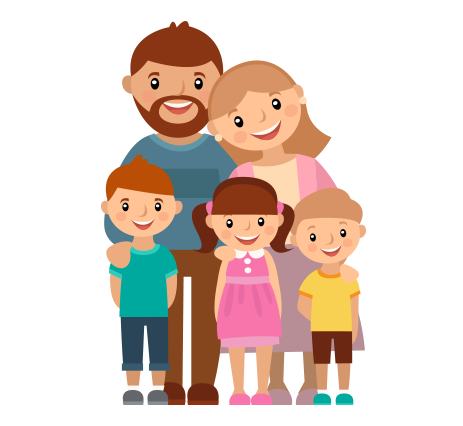
\includegraphics[scale=0.4]{imagenes/family.png}
		\caption{Integrantes de una Familia. (Elaboración Propia)}
		\label{family} 
		\end{figure}
	\section{Recursos de una vivienda}

\chapter{DESARROLLO DEL TRABAJO}

	\section{Introducción }
	El Problema que la mayoría de los desarrolladores enfrenta es el de como iniciar el desarrollo, ya teniendo las herramientas a utilizar y todo el cronograma planificado. Por ese motivo se describirá un proceso al cual realice unos ajustes para adecuarse a mis expectativas.
	
Para el desarrollo del sistema se optó por la utilización de un proceso de desarrollo denominado “proceso iterativo incremental” el cual se adecua de mejor manera  al modo de trabajo para este tipo de proyecto.
	\section{ Proceso de desarrollo de la metodología}
	Se realiza un análisis desde tres puntos de vista para entender mejor la estructura del sistema. La primera parte costa de un sistema de sensores y actuadores que están para el monitoreo de la vivienda.  La segunda parte es  el servidor y las comunicaciones entre el sistema de sensores/actuadores  y el cliente final, ya sea  haciendo uso de una red  local o una global como la internet. La 3º y última parte  que es la que el usuario final ve y hace uso de manera que le sea más  fácil la interacción con los recursos de la vivienda. Es el front-end que hace posible todo esto, ya que como el lenguaje web es multiplataforma hace más  sencillo a los usuarios finales el no tener q  instalar o depender de un sistema operativo en concreto para poder utilizar el sistema, gracias a esto los usuarios pueden acceder desde sus  PC,  portátiles con distintos tipos de sistemas operativos y mejor aún desde  sus Smartphone o tabletas.
	
El sistema de control domótica es realizado mediante 3 iteraciones los cuales son:
	\section{Sensores y Armado del Prototipo}
	La primera iteración consiste en la arquitectura del hardware, la recolección de datos mediante sensores y el envío de instrucciones a los activadores, dependiendo de las condiciones impuestas previamente. Los sensores almacenan la información en  variables para luego enviarlos al servidor en forma de una cadena.
	\subsection{Análisis}
	Analizando algunos escenarios para este módulo se vieron integrar las herramientas, dispositivos y tareas a consideradas para esta iteración:
	\begin{itemize}
	\item Herramientas.-  Se hace el uso del  IDE Arduino para la codificación y cargado del programa a la placa controladora. Para el ensamblado del prototipo es necesario: 
	\subitem Kit para el armado del PBC.
 	\subitem Conectores tipo hembra-macho.
	\subitem Conectores tipo macho-macho.
	\subitem Acrílico de 4mm de espesor para el diseño del case.
	\subitem Adaptador de AC de voltaje 220 con salida de 5v.
	\subitem Resistencias de 220ohm.
	\item Dispositivos.- Para el prototipo se vio conveniente el uso de los siguientes dispositivos: 
	\subitem Sensor de temperatura y humedad (DHT22).
	\subitem Sensor de detección de gas (MQ3). 
	\subitem Sensor de lluvia (YL-83). 
	\subitem Sensor de presencia (PIR).
	\subitem Módulo relé de 8 canales (para el manejo de corriente alterna).
	\subitem Modulo enchufe hembra.
	\subitem Led RGB de cátodo común.
	\item Tareas.- se realiza un cuadro de actividades con un orden de prioridades, las cuales se detallan en la Tabla  donde la primera columna pertenece a las actividades, la segunda la prioridad que tiene  estas y la tercera para la descripción detallada de la misma.
	
	\end{itemize}
	\begin{table}[ht]
			\begin{center} % tabla centrada en el texto
				\begin{tabular} {||l | c | p{8cm}||}
					\hline 
					\hline
					\multicolumn{3}{|c|}{Iteracion I: Hadware}\\
					\hline
					\hline 
					 Actividad & Prioridad & Descripcion \\   
					\hline
					\hline
					Preparación & 1 & Diagramación y armado de partes. \\  
					\hline
					Pruebas individuales & 2 &Pruebas de cada sensor y actuador . \\
					\hline
					Prueba conjunta & 2 & Pruebas de todos los sensores en un solo código Arduino. \\
					\hline
					Compra de hardware & 1 & Sensores y adquisición de equipo de electrónica.\\
					\hline
					Compactar hardware	& 3 & Fijar los componente de manera que sea portátil.\\
					\hline
					Construcción de case & 1 & Construcción de la caja para ensamblar los componentes.\\
					\hline
					Ensamblado & 1 & Ensamblado de sensores/actuadores  y todo los componentes necesarios.\\
					\hline
				\end{tabular}			
			\caption{Planificación de tareas primer módulo (Elaboración Propia).} 
			\label{tarea1}
			\end{center}
		\end{table}
		Pruebas década sensor  con las  librerías necesarias para el correcto funcionamiento esperando las salidas requeridas para el manejo de la información recolectada, A continuación se verán las pruebas con los sensores de temperatura y humedad DHT22, sensor de gas MQ2, sensor de presencia infrarroja PIR y el sensor de lluvia LY-83.
		
		\textbf{Temperatura y humedad:} Este sensor recolecta los cambios variantes en la temperatura y humedad del ambiente en el que se encuentra, se lo sitúa en habitaciones, sala de estar, dentro la vivienda para el monitoreo de cada sección de la misma. Es necesario la importación de dos librerías para el funcionamiento (DHT y Andafruitsensor) como se muestra en la Figura \ref{libsArduino}.
		\begin{figure}[ht]
		\centering
		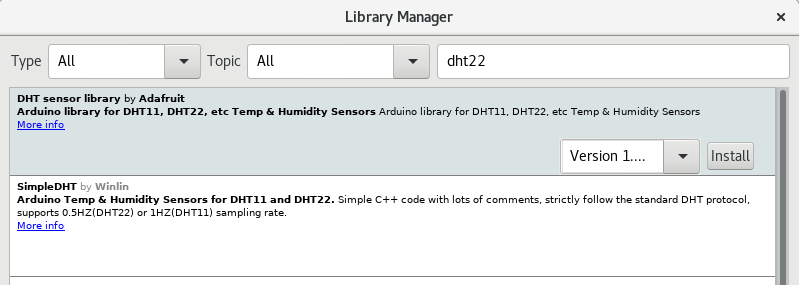
\includegraphics[scale=0.45]{imagenes/libsArduino.png}
		\caption{Libreria DHT22 para sensor de temperatura en Arduino IDE. (Elaboración Propia)}
		\label{libsArduino} 
		\end{figure}
		El código de lectura del sensor es por el pin 2 de manera digital, la librería nos facilita la conversión de los datos de entrada digital a la conversión de ºC y la lectura del valor de la humedad relativa. El resultado se lo puede observar en la Figura \ref{fig:temp}, la cual  muestra los valores que manda el sensor lo cual es visualizado por el monitor serial con los calores para temperatura= 26.40ºC y humedad del 34.60 \% respectivamente.
%		\begin{figure}[ht]
%		\centering
%		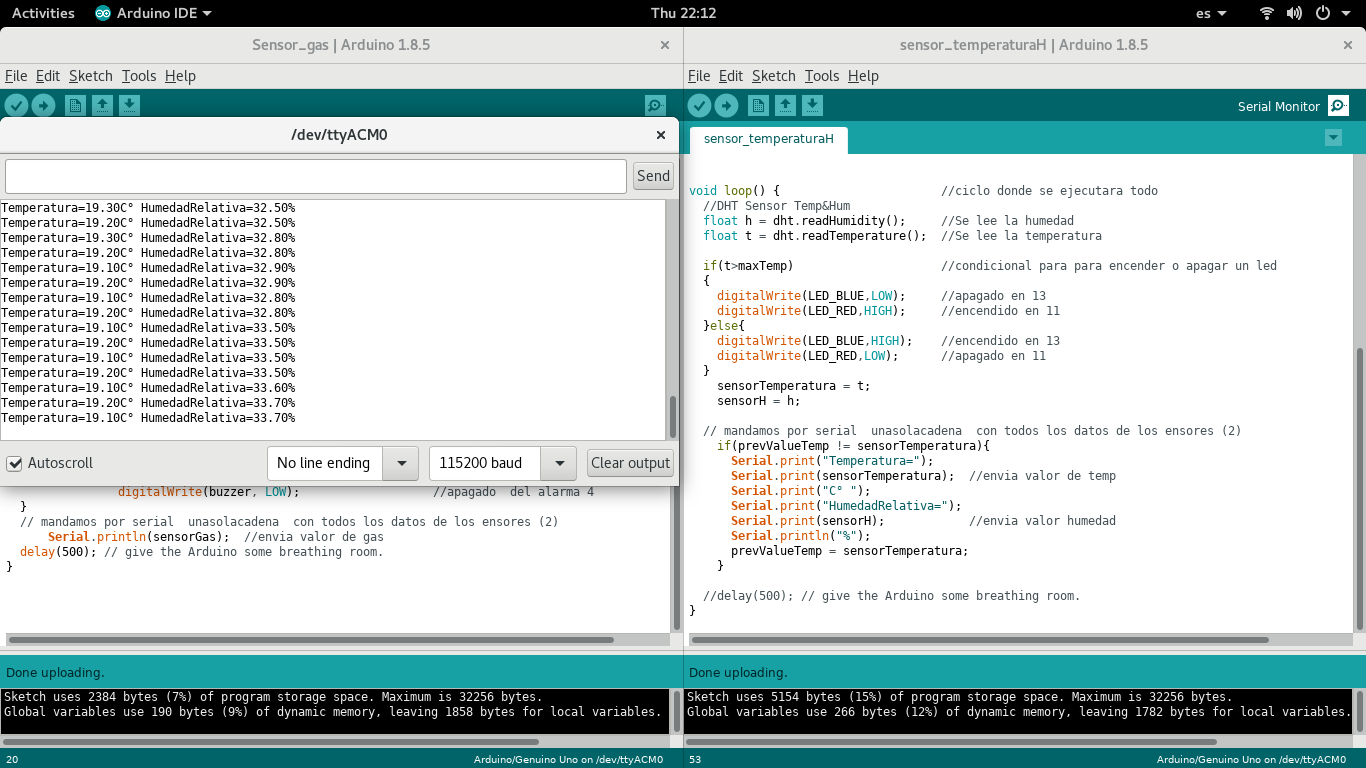
\includegraphics[scale=0.3]{imagenes/datosTemp.png}
%		\caption{Recolección de datos del sensor de Temperatura. (Elaboración Propia)}
%		\label{datosTemp} 
%		\end{figure}
		
		\textbf{Sensor de Gas MQ2:} Este sensor se lo sitúa en la cocina de mayor preferencia, de esta manera tener el monitoreo de esta área. La información que envía el sensor se recolecta  por el pin analógico A1 con valores de 1-1023 las cuales son mapeadas a valores de 0 a 100 para tener un mejor comprendiendo y relacionar a condiciones normales de los gases. La  cual define  que es dañino y peligroso si supera el valor de 30 y aceptable menor a esta.  En la Figura \ref{fig:gas} se muestra estados normales de concentración de gas con un valor de 2.
%		\begin{figure}[ht]
%		\centering
%		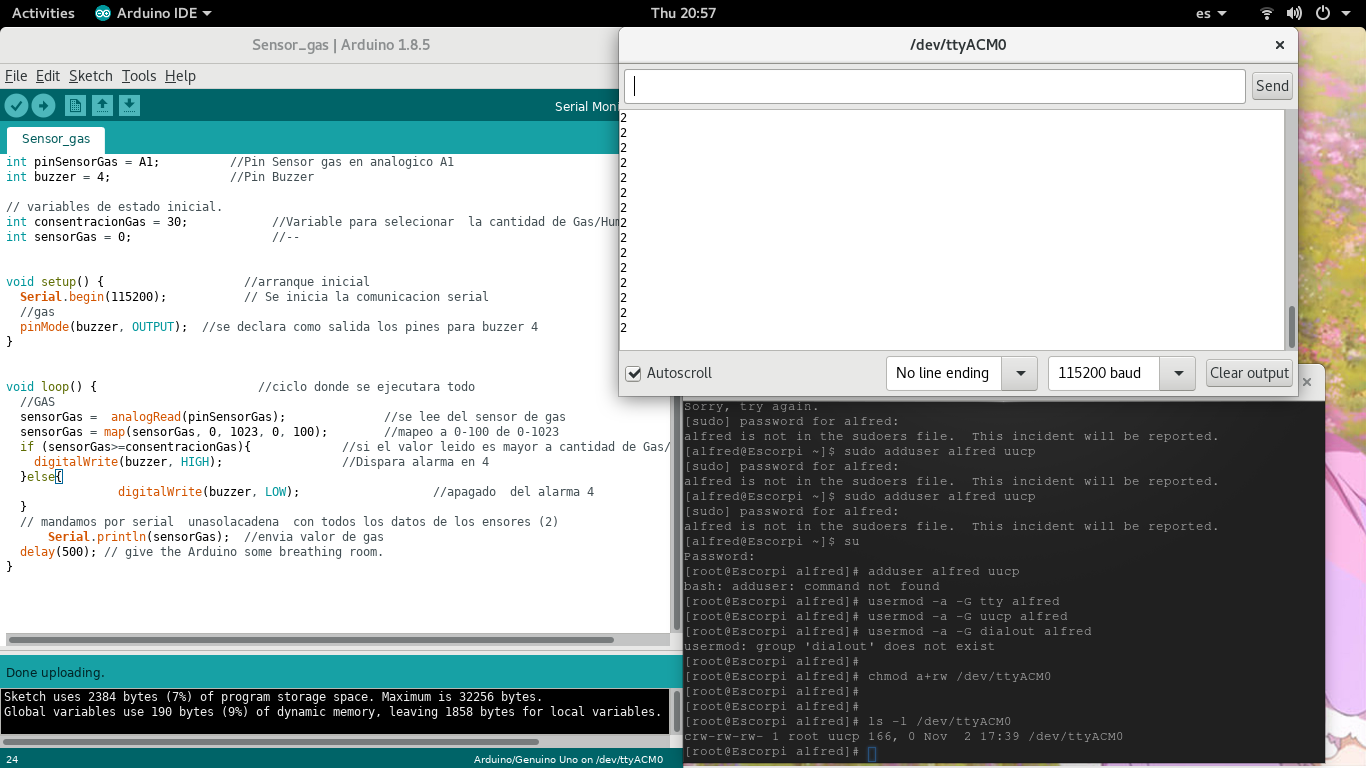
\includegraphics[scale=0.3]{imagenes/datosGas.png}
%		\caption{Recolección de datos del sensor de Gas MQ2. (Elaboración Propia)}
%		\label{datosGas} 
%		\end{figure}
		
		\textbf{Sensor de presencia PIR:} Este sensor de preferencia situado en los pasillos  para la activación de las luces, o en las puertas interiores, el sensor recoleta ondas de choque que varias en su entorno alrededor de 4-5 metros de distancia en un diámetro de aproximado 360º. Estas variaciones de ondas son regulables por el sensor para  ser más sensible o caso contrario, la variación de lectura de las ondas son  de 4s. En la Figura \ref{fig:pir} se puede apreciar la lectura  del cambio de estado del sensor el cual modifica un actuador Encendido/apagado respectivamente, en este caso cambia de un estado de apagado a encendido pasar una mano cerca del sensor.		
%		\begin{figure}[ht]
%		\centering
%		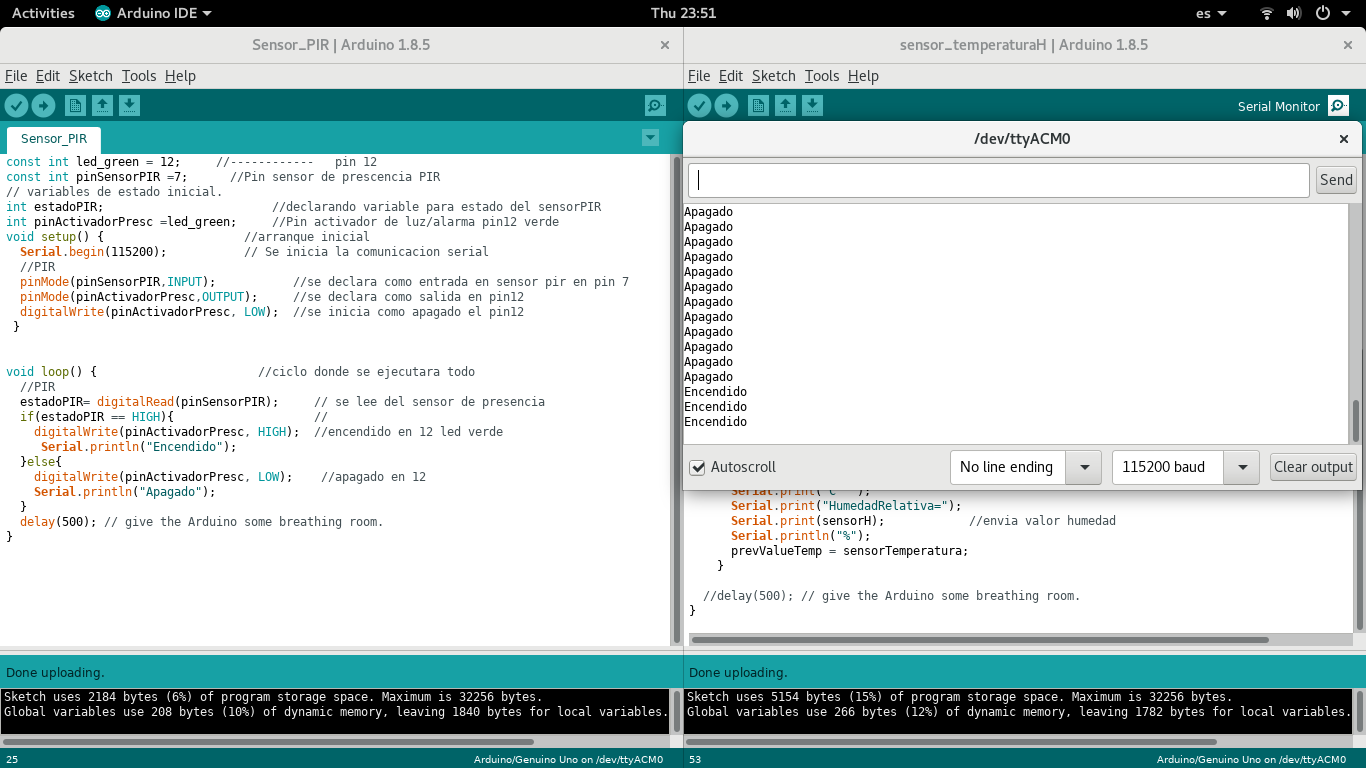
\includegraphics[scale=0.3]{imagenes/datosPIR.png}
%		\caption{Recolección de datos del sensor de presencia. (Elaboración Propia)}
%		\label{datosPIR} 
%		\end{figure}
			
		\textbf{Sensor de Lluvia YL-83:} de preferencia situarlo en la parte exterior de la vivienda, para recolectar información acerca de las lluvias. También puede actuar como sensor de fugas de agua. LA información es recolectada por el pin analógico A0, la cual está en un rango de valores de 0-1023 los cuales se mapean para que sea interpretada  de mejor manera en 0-100. En la Figura \ref{fig:lluvia} se muestra un cambio en los valores recolectados ya que se lo aplico agua en forma de gotas sobre el sensor, el cual reacciono de manera esperada.
		
%		\begin{figure}[ht]
%		\centering
%		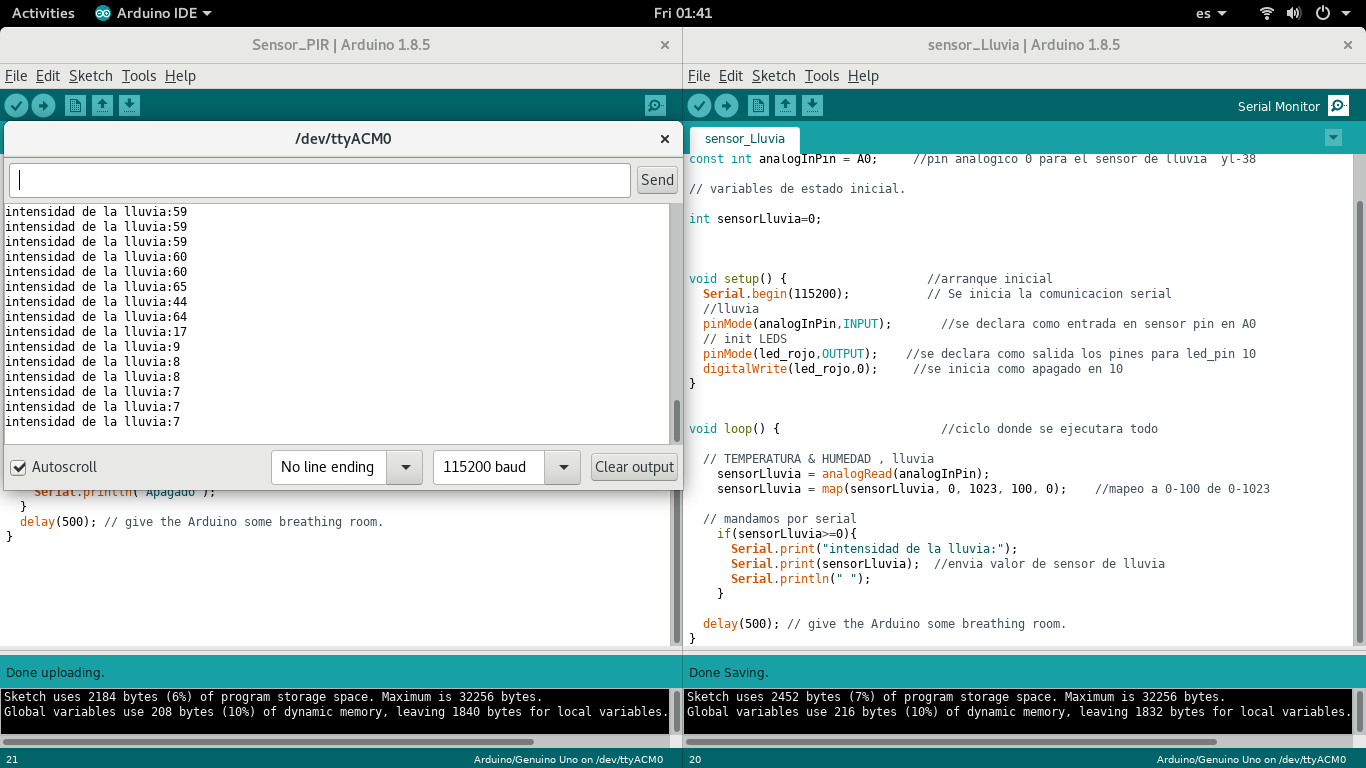
\includegraphics[scale=0.3]{imagenes/datosLluvia.png}
%		\caption{Recolección de datos del sensor de Lluvia. (Elaboración Propia)}
%		\label{datosLluvia} 
%		\end{figure}
% aqui van las  fuguras  de las  pruebas !
%sensores  firura
	\begin{figure}[ht]
    \centering
    \begin{subfigure}[b]{0.44\textwidth}
        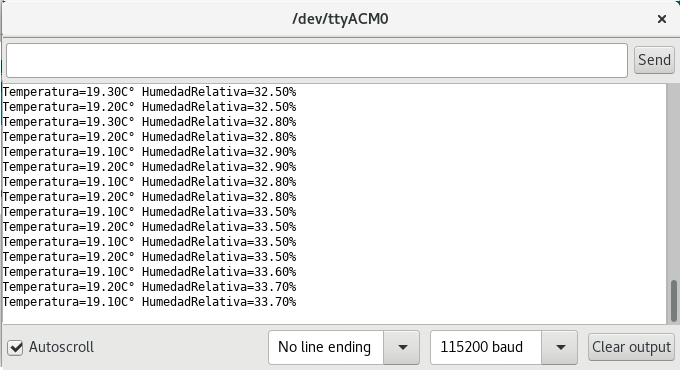
\includegraphics[width=\textwidth]{imagenes/datosTemp2.png}
        \caption{Recolección de datos del sensor de Temperatura. }
        \label{fig:temp}
    \end{subfigure}
    ~ %add desired spacing between images, e. g. ~, \quad, \qquad, \hfill etc. 
      %(or a blank line to force the subfigure onto a new line)
    \begin{subfigure}[b]{0.44\textwidth}
        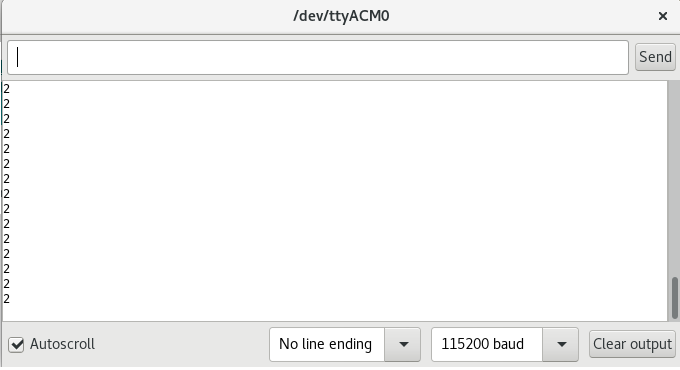
\includegraphics[width=\textwidth]{imagenes/datosGas2.png}
        \caption{Recolección de datos del sensor de Gas.}
        \label{fig:gas}
    \end{subfigure}
    ~ %add desired spacing between images, e. g. ~, \quad, \qquad, \hfill etc. 
    %(or a blank line to force the subfigure onto a new line)
    \begin{subfigure}[b]{0.44\textwidth}
        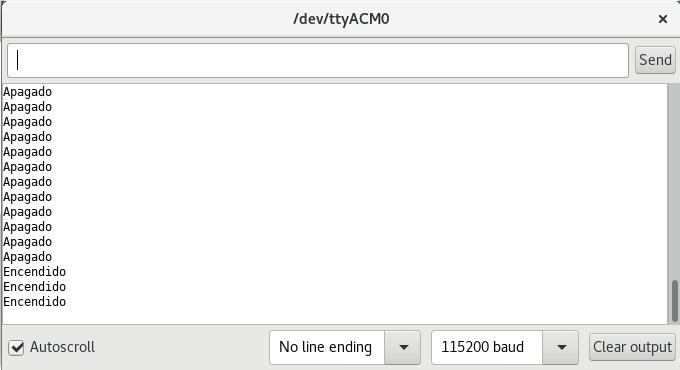
\includegraphics[width=\textwidth]{imagenes/datosPIR2.png}
        \caption{Recolección de datos del sensor de Proximidad. }
        \label{fig:pir}
    \end{subfigure}
     ~ %add desired spacing between images, e. g. ~, \quad, \qquad, \hfill etc. 
    %(or a blank line to force the subfigure onto a new line)
    \begin{subfigure}[b]{0.44\textwidth}
        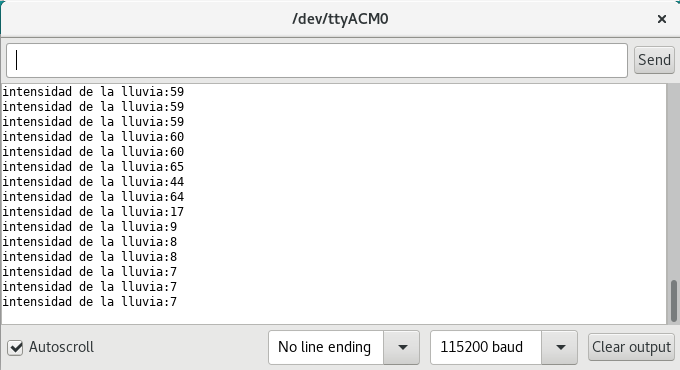
\includegraphics[width=\textwidth]{imagenes/datosLluvia2.png}
        \caption{Recolección de datos del sensor de Lluvia. }
        \label{fig:lluvia}
    \end{subfigure}
    \caption{Tipos de Vivienda Unifamiliar(Elaboración Propia)}\label{fig:sensores}
\end{figure}	

		\subsection{Diseño}
		Se realiza el diseño para el armado del prototipo, como también la integración con la siguiente iteración. El diseño se realiza mediante uso del framework fritzing, para poder tener una  interpretación más  certera, vease  la Figura \ref{fig:domotica_dis}.
%		\begin{figure}[h]
%		\centering
%		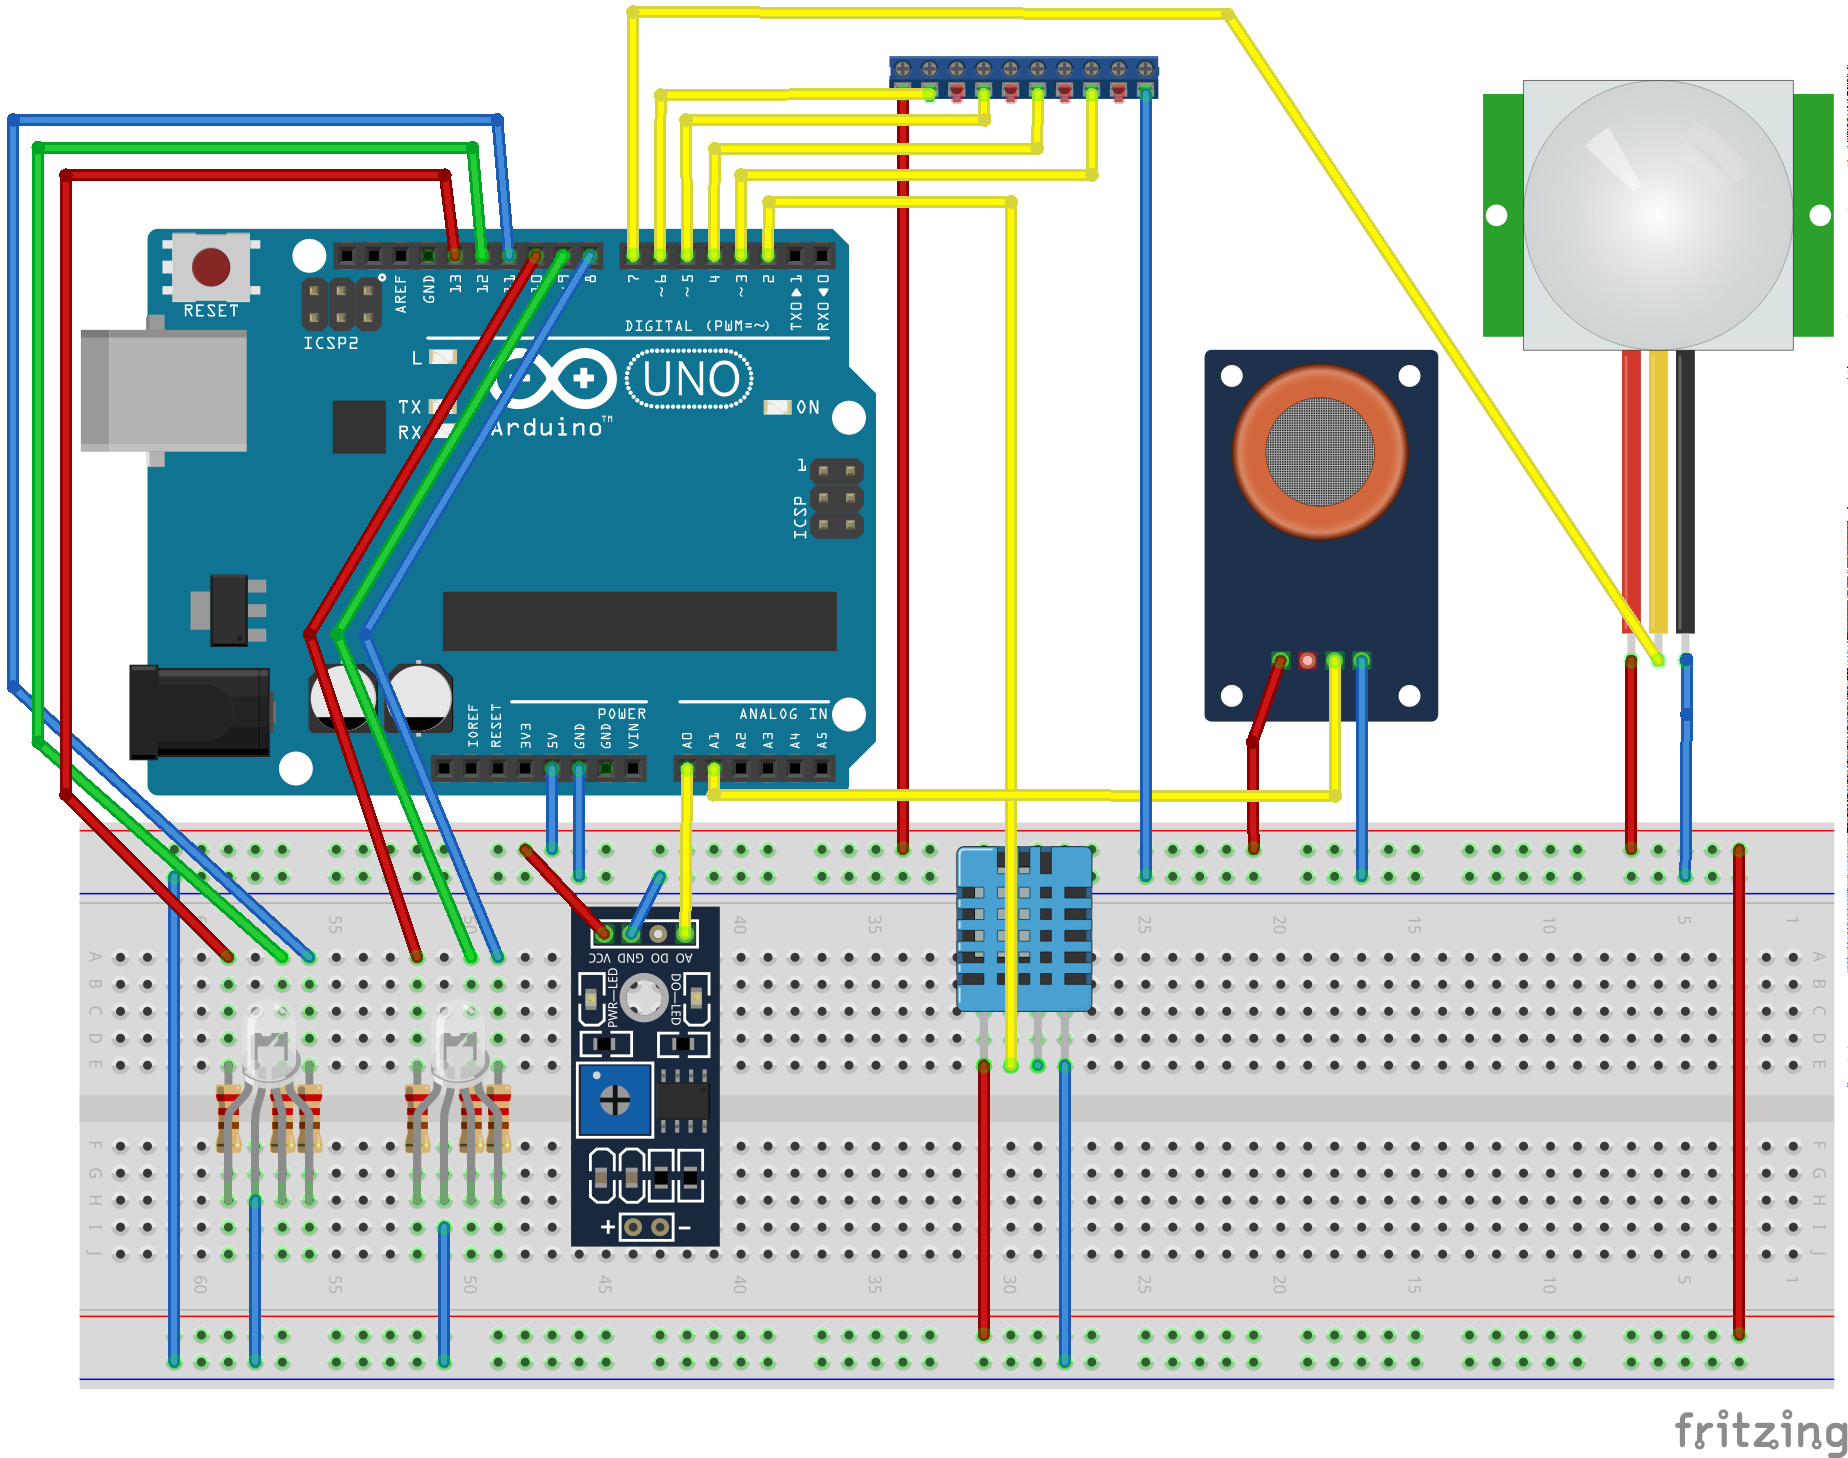
\includegraphics[scale=0.33]{imagenes/domotica_dis.png}
%		\caption{Diseño de los componentes en Fritzing. (Elaboración Propia)}
%		\label{domotica_dis} 
%		\end{figure}
		%diseño  firura
			\begin{figure}[htp]
   			 \centering
    			\begin{subfigure}[b]{0.3\textwidth}
      			  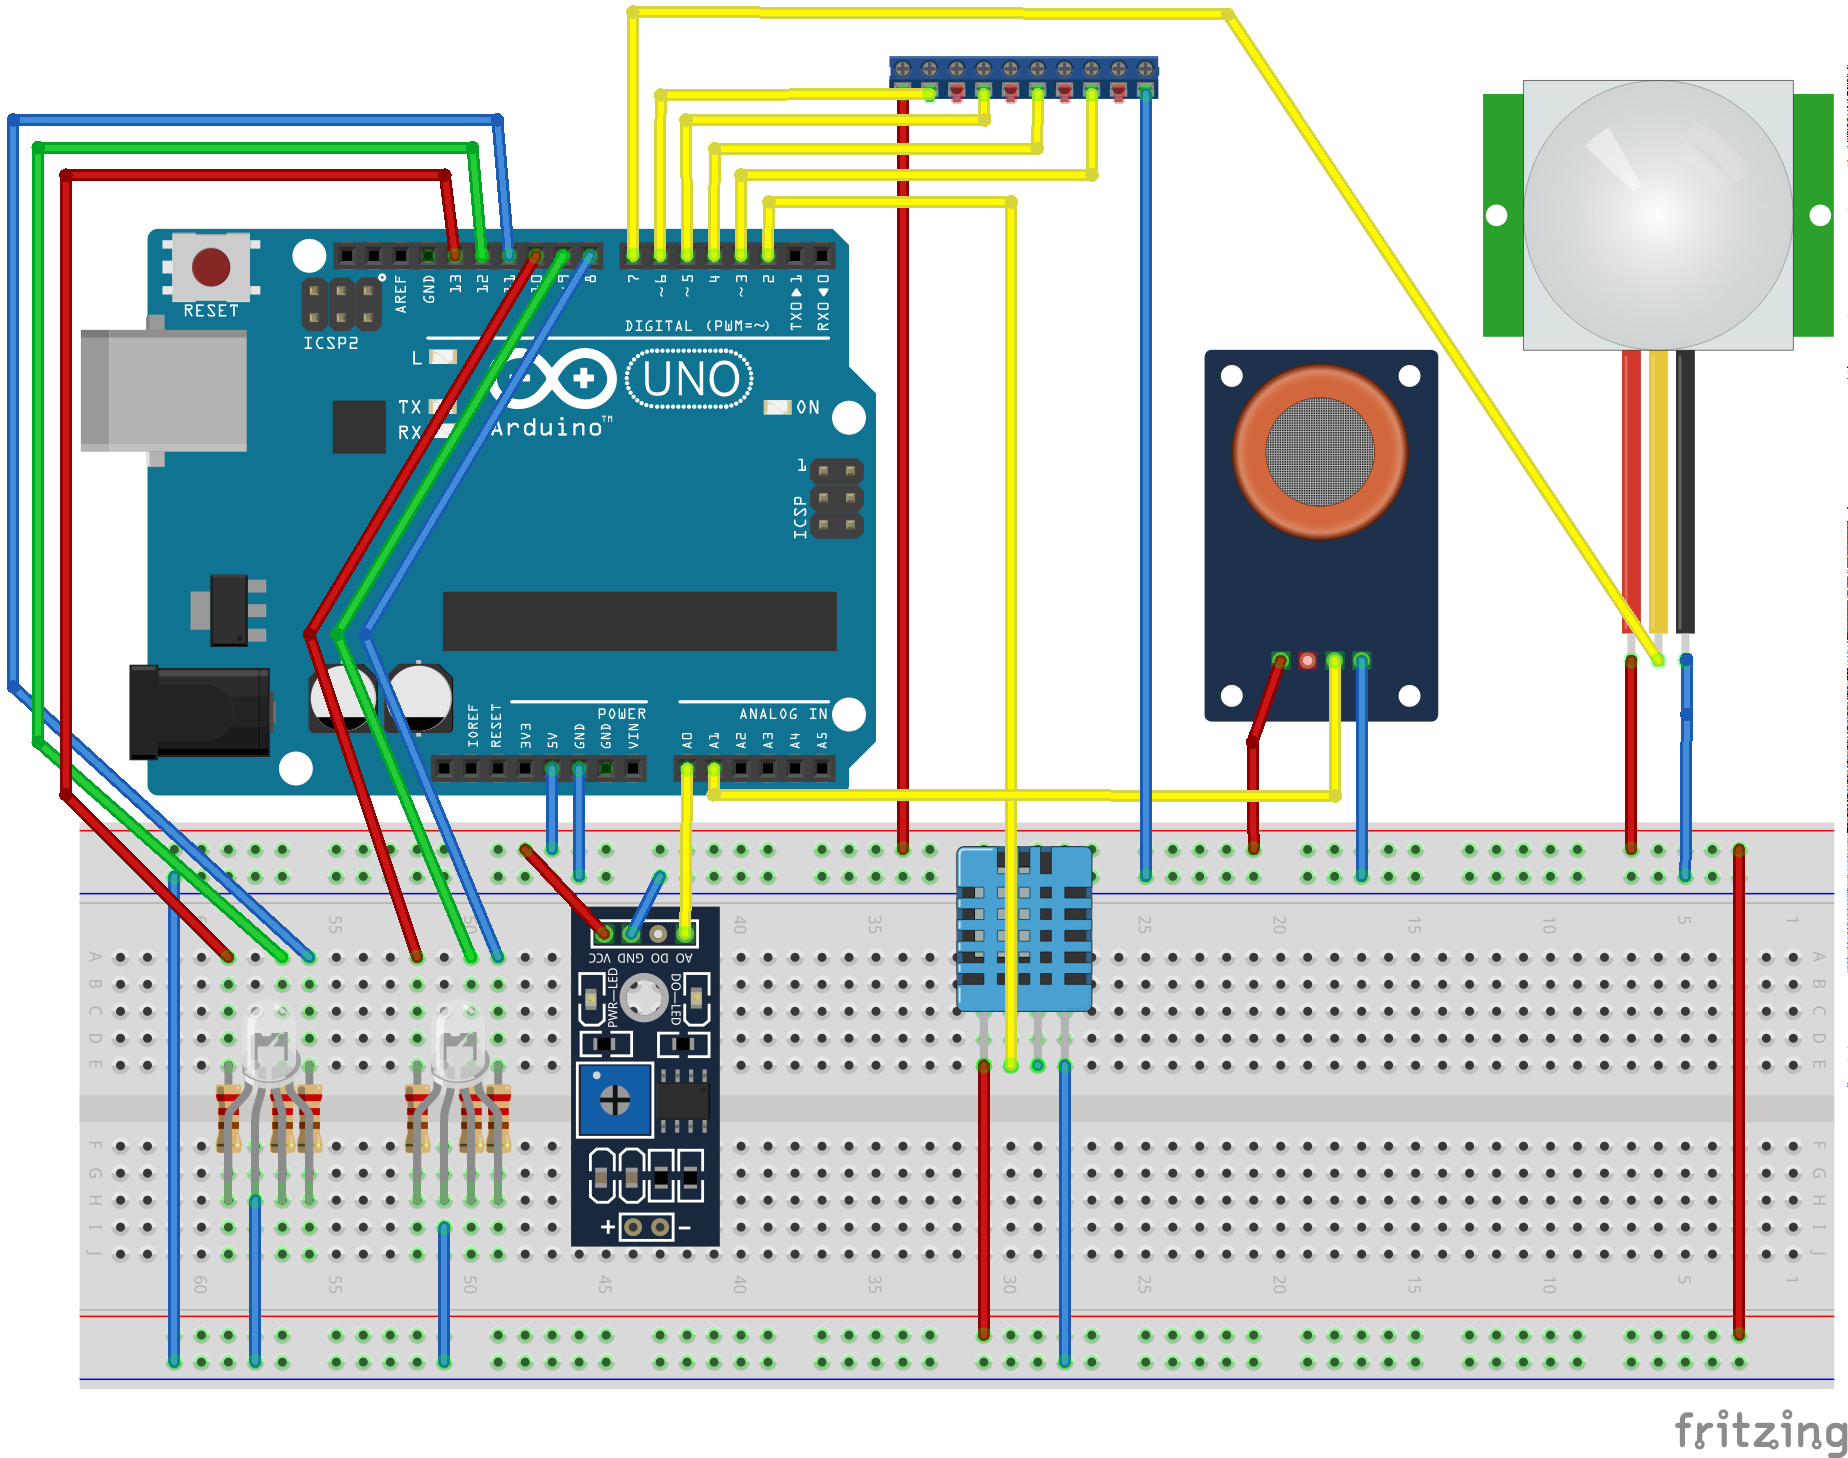
\includegraphics[width=\textwidth]{imagenes/domotica_dis.png}
        		\caption{Diseño de los componentes. }
       			 \label{fig:domotica_dis}
   				 \end{subfigure}
   				 \qquad %add desired spacing between images, e. g. ~, \quad, \qquad, \hfill etc. 
   				   %(or a blank line to force the subfigure onto a new line)
   				 \begin{subfigure}[b]{0.3\textwidth}
      			  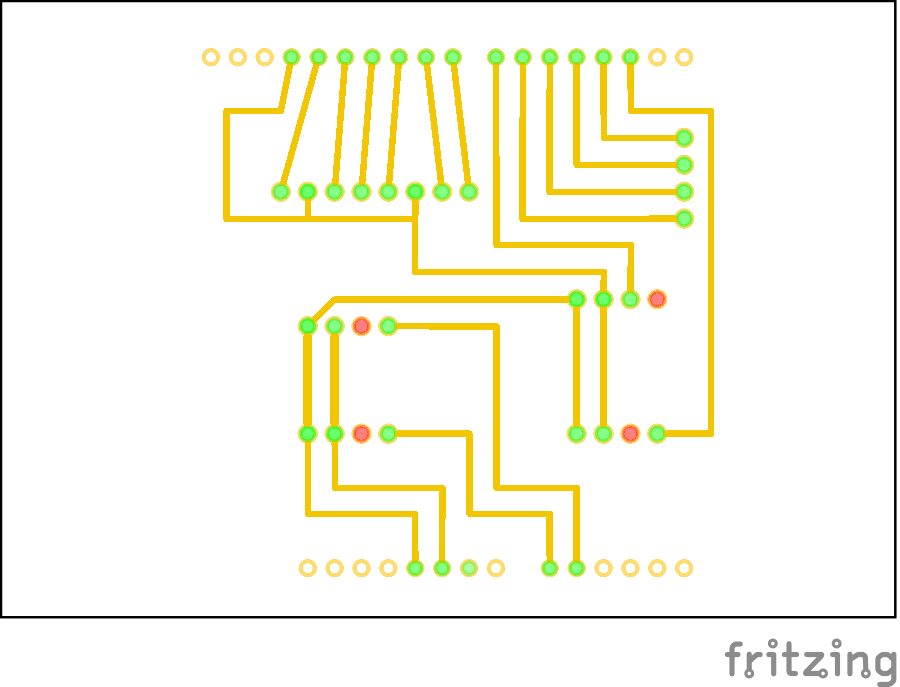
\includegraphics[width=\textwidth]{imagenes/dis_PP.png}
       		    \caption{Diseño de Placa de Prototipos.}
        	   	\label{fig:dis_PP}
   				 \end{subfigure}
   			 \caption{Diseño en Fritzing.(Elaboración Propia)}\label{fig:disenio}
			\end{figure}	
					
		Una vez terminado el diseño, se genera una placa de circuito como se ve en la Figura \ref{fig:dis_PP} , para el mejorar el encapsulado de los sensores y actuadores, para el que control y los demás hardware estén mejor situados.
%		\begin{figure}[h]
%		\centering
%		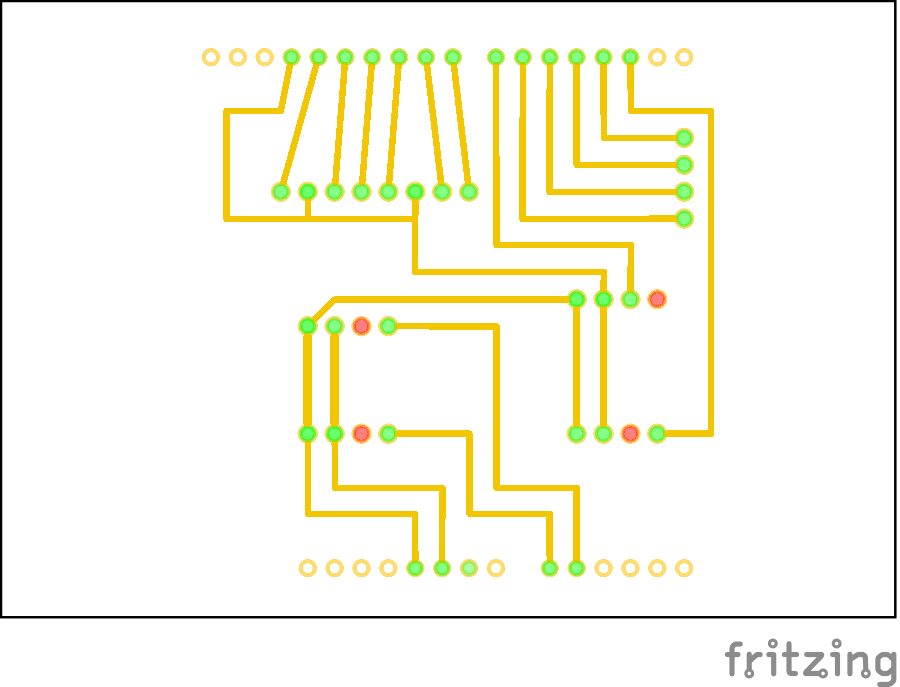
\includegraphics[scale=0.7]{imagenes/dis_PP.png}
%		\caption{Diseño de Placa de Prototipos. (Elaboración Propia)}
%		\label{dis_PP} 
%		\end{figure}
		
		Se realiza el diseño del case donde se encuentran los sensores y actuadores como también la placa controladora y la Raspberry. El diseño está realizada en Solidwork para corte láser en acrílico, teniendo como base  una dimensión de 20x23 cm. y los lados con cortes para los sensores y las placas, y una pata superior con perforaciones para los sensores de gas y presencia.
		Una vez terminado el diseño, se genera una placa de circuito como se ve en la Figura \ref{fig:dis_PP} , para el mejorar el encapsulado de los sensores y actuadores, para el que control y los demás hardware estén mejor situados.
		%case  firura
	\begin{figure}[ht]
    \centering
    \begin{subfigure}[b]{0.44\textwidth}
        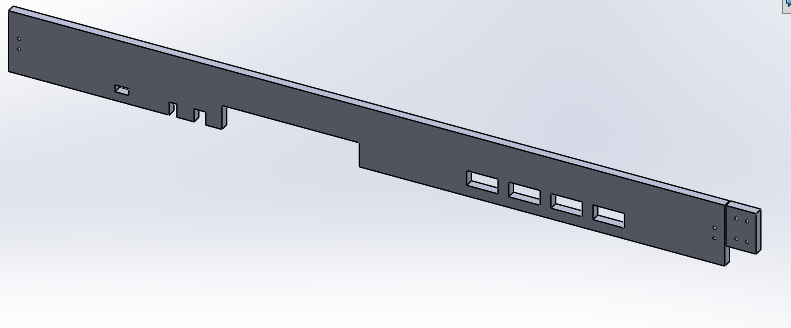
\includegraphics[width=\textwidth]{imagenes/bordes.png}
        \caption{Contorno del case. }
        \label{fig:bordes}
    \end{subfigure}
    ~ %add desired spacing between images, e. g. ~, \quad, \qquad, \hfill etc. 
      %(or a blank line to force the subfigure onto a new line)
    \begin{subfigure}[b]{0.44\textwidth}
        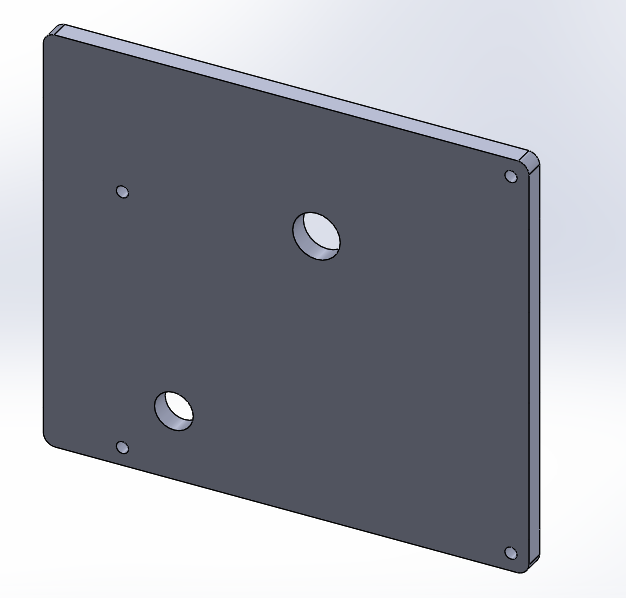
\includegraphics[width=\textwidth]{imagenes/tapa_arriba.png}
        \caption{Tapa del case.}
        \label{fig:arriba}
    \end{subfigure}
    \caption{Diseño del Case.(Elaboración Propia)}\label{fig:case}
\end{figure}
		
		
		
	\subsection{Codificación}
	El archivo principal para este módulo es “domotica.ino”. La  cual está realizado con el IDE Arduino, para poder apreciar  de mejor manera  ver el código completo en anexos.
Se importan las librerías necesarias de los sensores (DHT22)
%\begin{ArduinoSketchBox}{title}
%#include "DHT.h"          //cargamos la libreria DHT
%\end{ArduinoSketchBox}
		\begin{lstlisting}[language=Arduino]
			#include "DHT.h"          //cargamos la libreria DHT
		\end{lstlisting}
Luego se declara las variables y la inicialización de las mismas  como entradas digitales o analógicas, como los pines de salida. Todo esto en el método setup().
		\begin{lstlisting}[language=Arduino]
			Serial.begin(115200);     // Se inicia la comunicacion serial
		  dht.begin();              //Se inicia el sensor de temperatura y humedad
  		//Temperatura
  		pinMode(LED_RED, OUTPUT); //se declara como salida los pines para LED_RED 13
  		pinMode(LED_BLUE, OUTPUT);//se declara como salida los pines para LED_BLUE 11
  		//lluvia
  			pinMode(analogInPin,INPUT); //se declara como entrada en sensor pin en A0
  			//PIR
  			pinMode(pinSensorPIR,INPUT);    //se declara como entrada en sensor pin en pin 7
  			pinMode(pinActivadorPresc,OUTPUT);//se declara como salida en pin12
  			digitalWrite(pinActivadorPresc, LOW);//se inicia como apagado el pin12
  			//gas
  			pinMode(Rele, OUTPUT); //se declara como salida los pines para rele 3
  			pinMode(buzzer, OUTPUT);//se declara como salida los pines para buzzer 4
  			pinMode(agua, OUTPUT); //se declara como salida los pines para agua 5
  			// init LEDS
  			pinMode(led_rojo,OUTPUT); //se declara como salida los pines para led_pin 10
  			pinMode(led_verde,OUTPUT);//se declara como salida los pines para pwmPin 9
  			pinMode(led_azul,OUTPUT); //se declara como salida los pines para pin 8
		\end{lstlisting}
Y las funciones más importantes en el control y manejo de información recolectado por los sensores son las siguientes que están dentro de la función loop():

		\begin{lstlisting}[language=Arduino]
		//DHT Sensor Temp&Hum
		float h = dht.readHumidity();     //Se lee la humedad
		float t = dht.readTemperature();  //Se lee la temperatura
		//PIR
		estadoPIR= digitalRead(pinSensorPIR);    // se lee del sensor PIR
		//GAS
		sensorGas =  analogRead(pinSensorGas);   //se lee del sensor de gas
		sensorGas = map(sensorGas, 0, 1023, 0, 100); //mapeo de 0-100 de 0-1023
		\end{lstlisting}
La obtención de instrucciones que se recibe por medio del servidor es de forma alfanumérica (a1), donde la letra es la clave que hace referencia a un actuador seguida de un valor, la cual es la instrucción que realizara en este caso el encendido (1) y apagado (0).
		\begin{lstlisting}[language=Arduino]
		 //  lee una letra y que recoja el valor
        if(Serial.available()>0){
    	lectura = Serial.read();  
    	switch (lectura) {
    	case 'a':
       	lectura = Serial.parseInt();
       	digitalWrite(led_azul,lectura);
      	break;
   		 default: 
    	break;
 		 }
		\end{lstlisting}

Los datos recolectados por los sensores son enviados en forma de cadena al servidor mediante comunicación serial:
		\begin{lstlisting}[language=Arduino]
			// mandamos por serial  una sola cadena  con todos los datos de los sensores 
		    if(prevValueTemp != sensorTemperatura){
		      Serial.print("B");                // inicio de caracter 
		      Serial.print(sensorTemperatura);  //envia valor de temp
		      Serial.print(" ");            //separador de cadenas para el split
		      Serial.print(sensorGas);            //envia valor GAS
		      Serial.print(" ");            //separador de cadenas para el split
		      Serial.print(sensorH);            //envia valor humedad
		      Serial.println("E");              // fin del caracter
		      prevValueTemp = sensorTemperatura;
		}
		\end{lstlisting}

	\subsection{Pruebas}
	Para validar el correcto funcionamiento y la calidad en esta iteración se realizan las pruebas de caja blanca y caja negra:
	\begin{itemize}
	\item Pruebas de Caja Negra.- Se realizaron las pruebas tanto en cada sensor de forma individual como de forma conjunta para  poder recolectar los datos y  enviarlos por comunicación serial. En la Figura \ref{fig:salida1} se muestra los valores “B21.00 12 35.80E” estos valores corresponden a la temperatura, concentración de gas y la humedad respectivamente. El envío de datos ocurre siempre y cuando hay una variación en el valor de los sensores leídos anteriormente comparados con la lectura actual.
	\item Pruebas de Caja Blanca.- Como se vi anteriormente uno de las funciones importantes es el  envío de datos por comunicación serial que se realiza mediante el siguiente método de forma correcta vease la Figura \ref{fig:flujo1}. 
	\end{itemize}
		%case  firura
	\begin{figure}[ht]
    \centering
    \begin{subfigure}[b]{0.4\textwidth}
        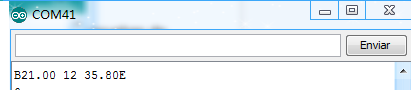
\includegraphics[width=\textwidth]{imagenes/salida.png}
        \caption{Salida de Datos por el Puerto Serial. }
        \label{fig:salida1}
    \end{subfigure}
    ~ %add desired spacing between images, e. g. ~, \quad, \qquad, \hfill etc. 
      %(or a blank line to force the subfigure onto a new line)
    \begin{subfigure}[b]{0.5\textwidth}
        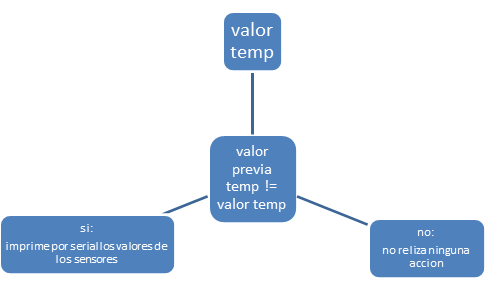
\includegraphics[width=\textwidth]{imagenes/flujo.png}
        \caption{Flujo de datos de la Funcion de envio de datos.}
        \label{fig:flujo1}
    \end{subfigure}
    \caption{Pruebas de Caja Negra y Blanca.(Elaboración Propia)}\label{fig:pruebasI}
\end{figure}


	\section{Montar servidor  NodeJS y Establecer Comunicaciones}
	Esta es la segunda iteración que se encarga de establecer la comunicación entre la parte del hardware donde se encuentran los sensores/actuadores y la placa controladora. Mediante una comunicación serial es posible establecer la conexión con el servidor que se encuentra  en una Raspberry. Cabe recalcar que la comunicación serial está ligada al hardware y no pueden estar separadas más de 2m de distancia de la placa controladora.
Para la realización de esta iteración se vio necesario seguir las siguientes acciones:

		% Para trabajar con tablas sugiero utilizar Macro Excel2Latex (ver carpeta útiles)
		% La tabla siguiente tiene dos columnas y se indican con '{l c}'
	\subsection{Análisis}
	Se realiza la planificación de las tareas de este módulo  como la recolección de requerimientos y generar plan de trabajo como se muestra en la Tabla .
	
%		\begin{table}[h]
%			\begin{center} % tabla centrada en el texto
%				\begin{tabular} {||l | c | l||}%l -> left, c -> center, r -> right
%					\hline % línea horizontal
%					\hline 
%					 Actividad & Prioridad & Descripción \\  % Fila de encabezados 
%					\hline
%					\hline
%					Preparación & 1 & Diseño de  mockups. \\  % (\\ indica el final de la línea)
%					\hline
%					Control encendido/apagado & 1 &Acciones de encendido/apagado desde la web. \\
%					\hline
%					Comunicación con el servidor & 1 & usar sockects con el servidor. \\
%					\hline
%					Cámaras & 3 & Vistas para las cámaras.\\
%					\hline
%					Monitoreo	& 1 & Vistas de los datos de los sensores.\\
%					\hline
%					Grafica & 3 & representacion  de datos en grafica.\\
%					\hline
%					Simulacion de prescencia & 2 & Acciones programadas de encendido/apagado durante el dia y  la noche.\\
%					\hline
%				\end{tabular}
			
%			\caption{Planificación de tareas (Elaboración Propia).} 
%			\label{tablaDos}
	     % label: etiqueta tabla, sirve para ref. cruzadas, ver video: 
    	 % https://www.youtube.com/watch?v=ldU2mEWAeh4
%			\end{center}
%		\end{table}
	\begin{table}[H]
			\begin{center} % tabla centrada en el texto
				\begin{tabular} {||l | c | p{8cm}||}
					\hline 
					\hline
					\multicolumn{3}{|c|}{Iteracion II: Servidor}\\
					\hline
					\hline 
					 Actividad & Prioridad & Descripcion \\   
					\hline
					\hline
					Preparación & 1 & Configuración del router. \\  
					\hline
					Configurar Raspberry & 2 &Instalación de NodeJS y dependencias. \\
					\hline
					Scaffold & 1 & Creación de la estructura  del servidor. \\
					\hline
					Comunicación serial  & 1 & Recolección/envió de datos por serial con el Arduino.\\
					\hline
					Ip publica	& 3 & Definir la ip publica para el acceso al servidor desde internet.\\
					\hline
					Control de tiempos & 1 & Control de tiempos de respuesta desde un cliente al hardware.\\
					\hline
					Acceso remoto & 2 & Configuración de servicio VNC y ssh.\\
					\hline
				\end{tabular}			
			\caption{Planificación de tareas Segundo Módulo (Elaboración Propia).} 
			\label{tarea2}
			\end{center}
		\end{table}
		\subsection{Diseño}
		La parte del sistema de los sensores recolecta toda la información necesaria y los envía por comunicación serial protocolo rc3220 hacia el servidor  de node. El cual recolecta esa información y  actualiza todos los datos de los sensores y los muestras a todos  los usuarios conectados mediante el modulo socket.io, este último es para aplicaciones en tiempo real, la cual hace posible que cada cambio realizado por un usuario sea visible al  mismo tiempo por otros que están conectados al mismo tiempo o ver los cambios  al ingresar al sistema. Para que el sistema de los sensores tenga mayor certeza en los tiempos es necesario que se encuentren en una  misma red local tanto el servidor como el sistema de sensores.
		\begin{figure}[H]
		\centering
		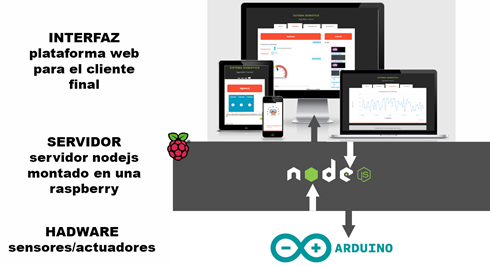
\includegraphics[scale=0.9]{imagenes/arquitectura.png}
		\caption{Diseño del Esquema de Comunicación Entre los Módulos.}
		 Fuente:(Elaboración Propia)
		\label{modulos} 
		\end{figure}
El diseño para una infraestructura de aplicaciones web de NodeJS se realiza mediante herramienta de generador de aplicaciones express para crear rápidamente un esqueleto de aplicación. La aplicación generada tiene la siguiente estructura de directorios:
		\begin{figure}[ht]
		\centering
		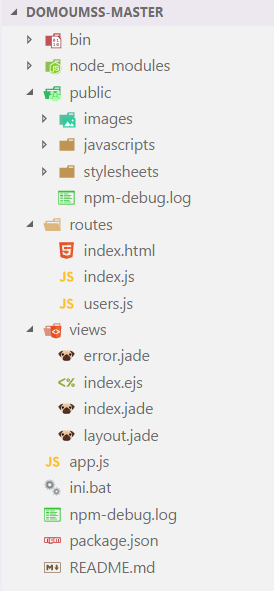
\includegraphics[scale=0.7]{imagenes/arbol_directorios.png}
		\caption{Diseño del Árbol Directorios.}
					Fuente(Elaboración Propia)
		\label{arbol_directorios} 
		\end{figure}

	\subsection{Codificación}
	Los módulos principales para la comunicación entre el Arduino y el servidor, como también el servidor y los usuarios finales mediante la plataforma web  se requiere de estos dos módulos: serialport y socket.io. Para esto se instala el módulo utilizando el gestor de paquetes de Nodejs 


		\begin{figure}[ht]
			\centering
			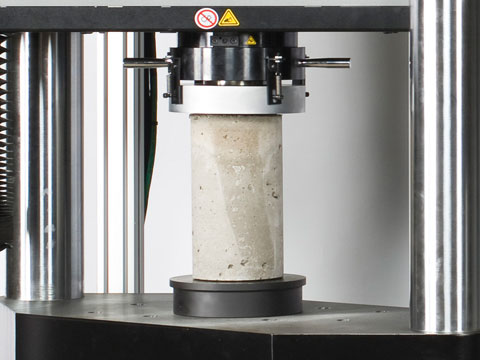
\includegraphics[scale=0.5]{imagenes/ASTM_C39_image1.jpg}
			\caption{Probeta hormigón (Autor, año)}
			\label{probetaHormigon} 
			% Label: es para realizar referencias cruzadas, 
			% notar que se escribe todo junto y sin acentos.
		\end{figure}

	La Figura \ref{probetaHormigon} Muestra ... (Explicar las figuras. Notar que la figura fue
	citada con referencia cruzada y la numeración es automática) 
	
	%% Ver video referencias cruzadas: https://www.youtube.com/watch?v=ldU2mEWAeh4


\chapter{Resultados.} 

	
	\section{Ejemplo de titulo 2.}
		
		\subsection{Ejemplo de titulo 3.}
			
			\subsubsection{Ejemplo de titulo 4 (no numerado).}

				\paragraph{Ejemplo de título 5:}

								
	\section{Discusión de resultados.}


\chapter{Conclusiones}





%%%%%%%%%%%%%%%%%%%%%%%%%%%%%%%%%%%%%%%%%%%%%%%%%%%%%%%%%%%%%%%%%%%%%%%%%%%%%%%%%%%%%%%%%%%%%%%%%
%%%%%%%%%%%%%%%%%%%%%%%%%%%%%%%%%%%% Bibliografía %%%%%%%%%%%%%%%%%%%%%%%%%%%%%%%%%%%%%%%%%%%%%%%
%%%%%%%%%%%%%%%%%%%%%%%%%%%%%%%%%%%%%%%%%%%%%%%%%%%%%%%%%%%%%%%%%%%%%%%%%%%%%%%%%%%%%%%%%%%%%%%%%
	
	% Para aprender a usar la bibliografía ver el siguiente video:
 	% https://www.youtube.com/watch?v=MnL5dI41IOA

	% No modificar esta sección
 
	\renewcommand{\refname}{Bibliografía} % Bibliografía en español
	\addcontentsline{toc}{chapter}{Bibliografía} % Agrega la bibliografía al Índice.
	\bibliographystyle{apalike} % formato APA 

	\bibliography{perifericos/bibliografia} 


%%%%%%%%%%%%%%%%%%%%%%%%%%%%%%%%%%%%%%%%%%%%%%%%%%%%%%%%%%%%%%%%%%%%%%%%%%%%%%%%%%%%%%%%%%%%%%%%%
%%%%%%%%%%%%%%%%%%%%%%%%%%%%%%%%%%%% Anexos o apéndices %%%%%%%%%%%%%%%%%%%%%%%%%%%%%%%%%%%%%%%%%
%%%%%%%%%%%%%%%%%%%%%%%%%%%%%%%%%%%%%%%%%%%%%%%%%%%%%%%%%%%%%%%%%%%%%%%%%%%%%%%%%%%%%%%%%%%%%%%%%


	% El siguiente archivo conntiene los apéndices
	% Está en un archivo diferente para que el presente archivo sea menos extenso.
	% En caso de no existir anexos simplemente eliminar o anteponer '%'
	
\appendix

\chapter{Ejemplo de apéndice o anexo}

\section{Sub título primer apéndice o anexo}



\subsection{Sub sección del primer apéndice o anexo}




\end{document}